\documentclass[xcolor=table]{beamer}
\usetheme{default}
\usecolortheme{wolverine}
\usepackage{subfigure}
\usepackage{graphicx}
\usepackage{tabularx}
\usepackage{booktabs}
\usepackage{ragged2e}
\usepackage{caption}
\usepackage{adjustbox}


\setbeamercolor{normal text}{fg=white}
\setbeamercolor{caption name}{fg=yellow}
\definecolor{mybg}{RGB}{2, 61, 150}
\setbeamercolor{background canvas}{bg=mybg}
\setbeamercolor{itemize item}{fg=yellow}
\setbeamercolor{itemize item}{fg=yellow}
\setbeamercolor{itemize subitem}{fg=yellow}
\setbeamercolor{itemize subsubitem}{fg=yellow}
\setbeamertemplate{caption}{\color{yellow}\insertcaption}

\usefonttheme{professionalfonts}
\setbeamerfont{frametitle}{size=\large}
\setbeamerfont{normal text}{size=\large}

\beamertemplatenavigationsymbolsempty

\title{D.S.P. based Field Oriented Control of Induction motor}
\author{Adhithya S 200901002\\Anabhayan S P 200901008}
\date{Under the guidance of Dr S Rama Reddy \\ Dean - Electrical sciences \vspace{0.3in}\\                  {\small\textit{Department of Electrical and Electronics Engineering\\Rajalakshmi Engineering college}}}

\usepackage{tikz}

\usetikzlibrary{shapes.geometric, arrows}

\setbeamercolor{itemize item}{fg=yellow}
 % Keep your preamble

\begin{document}

% Slide 1: Title Slide (keep as is)
\begin{frame}{}
	\maketitle
\end{frame}


\begin{frame}{DC Motor Control Loop}
	\begin{figure}
		\centering
		\fbox{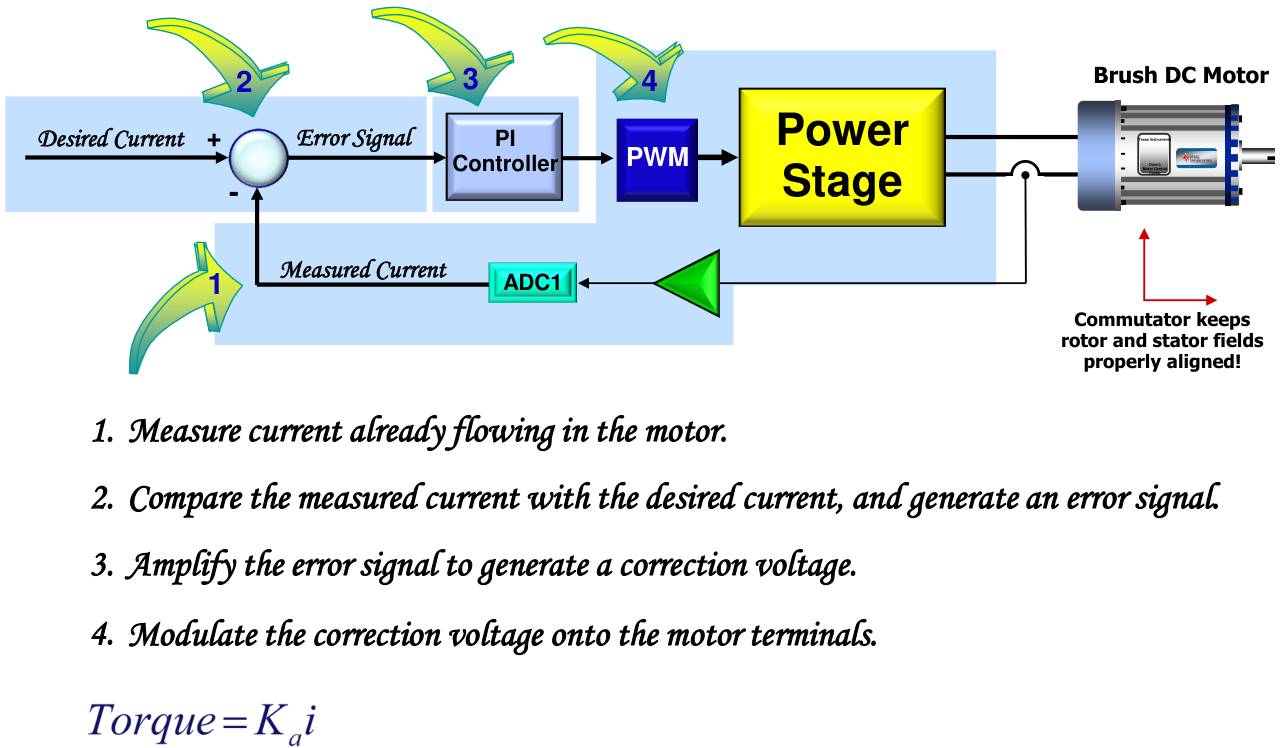
\includegraphics[width=4in]{sections/finalReview/dcMotor.png}}
		\caption{Commutator naturally adjust for MTPA}
	\end{figure}
\end{frame}


\begin{frame}{Field Oriented Control in a Nutshell}
	\begin{figure}
		\centering
		\fbox{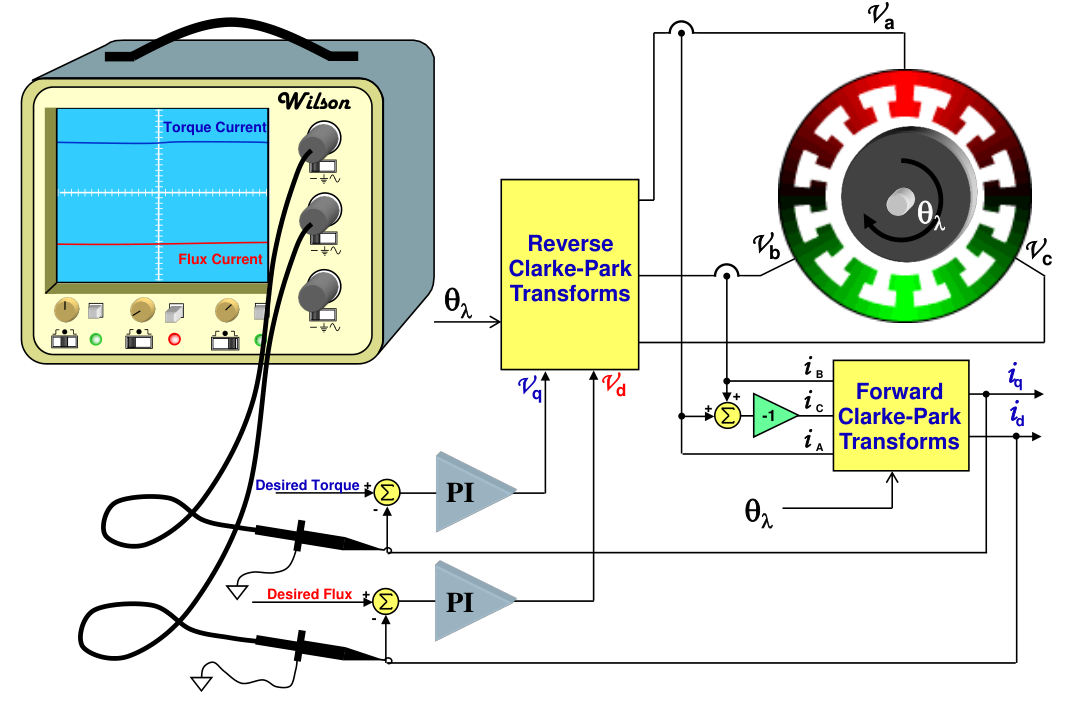
\includegraphics[width=4in]{sections/finalReview/focCoreSimply.png}}
		\caption{Field Oriented Control in a Nutshell}
	\end{figure}
\end{frame}
% Slide 2: Block Diagram of FOC
\begin{frame}{Block Diagram of Field Oriented Control}
	\begin{figure}
		\centering
		\fbox{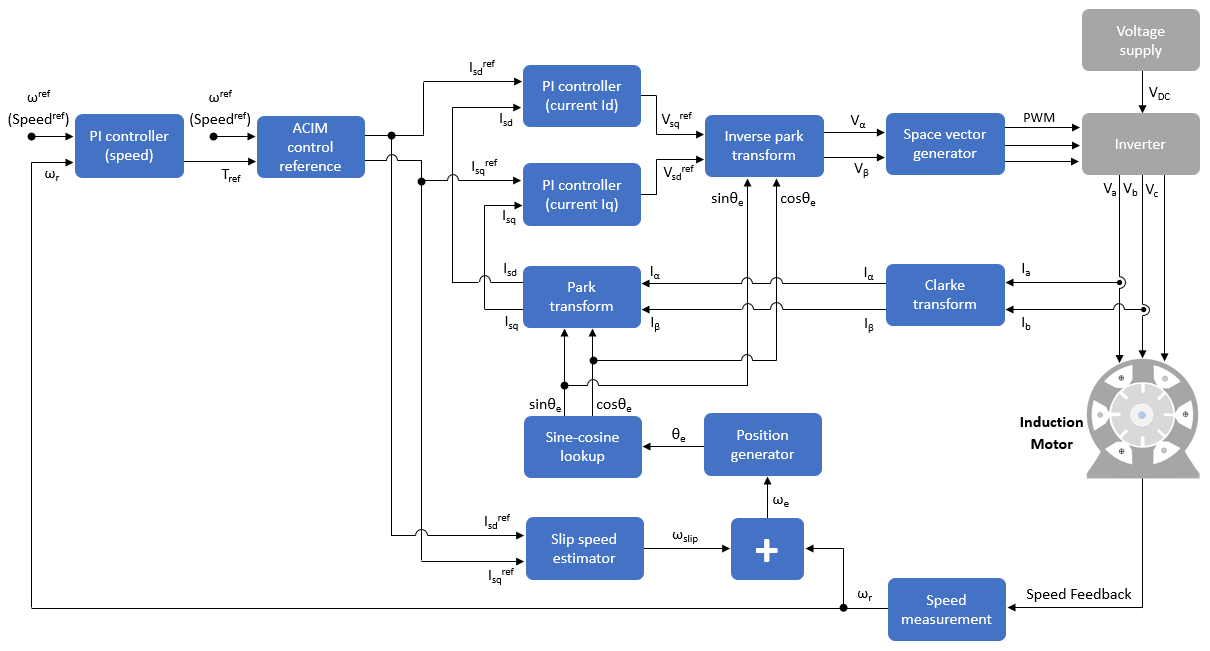
\includegraphics[width=3in]{sections/section2/images/blockDiagram.png}}
		\caption{Block Diagram of Field Oriented Control}
	\end{figure}
	\begin{itemize}
		\item Actual Current.
		\item Reference Current.
		\item PWM Generation.
		\item Rotor Flux Estimation.
	\end{itemize}
\end{frame}

% coordinate transform images

\begin{frame}{Coordinate Transformations}
	\begin{itemize}
		\item RMF Animation
		\item Clark Animation
		\item Park Animation
	\end{itemize}
\end{frame}


\begin{frame}{Coordinate Transformations}
	\begin{figure}
		\centering
		\fbox{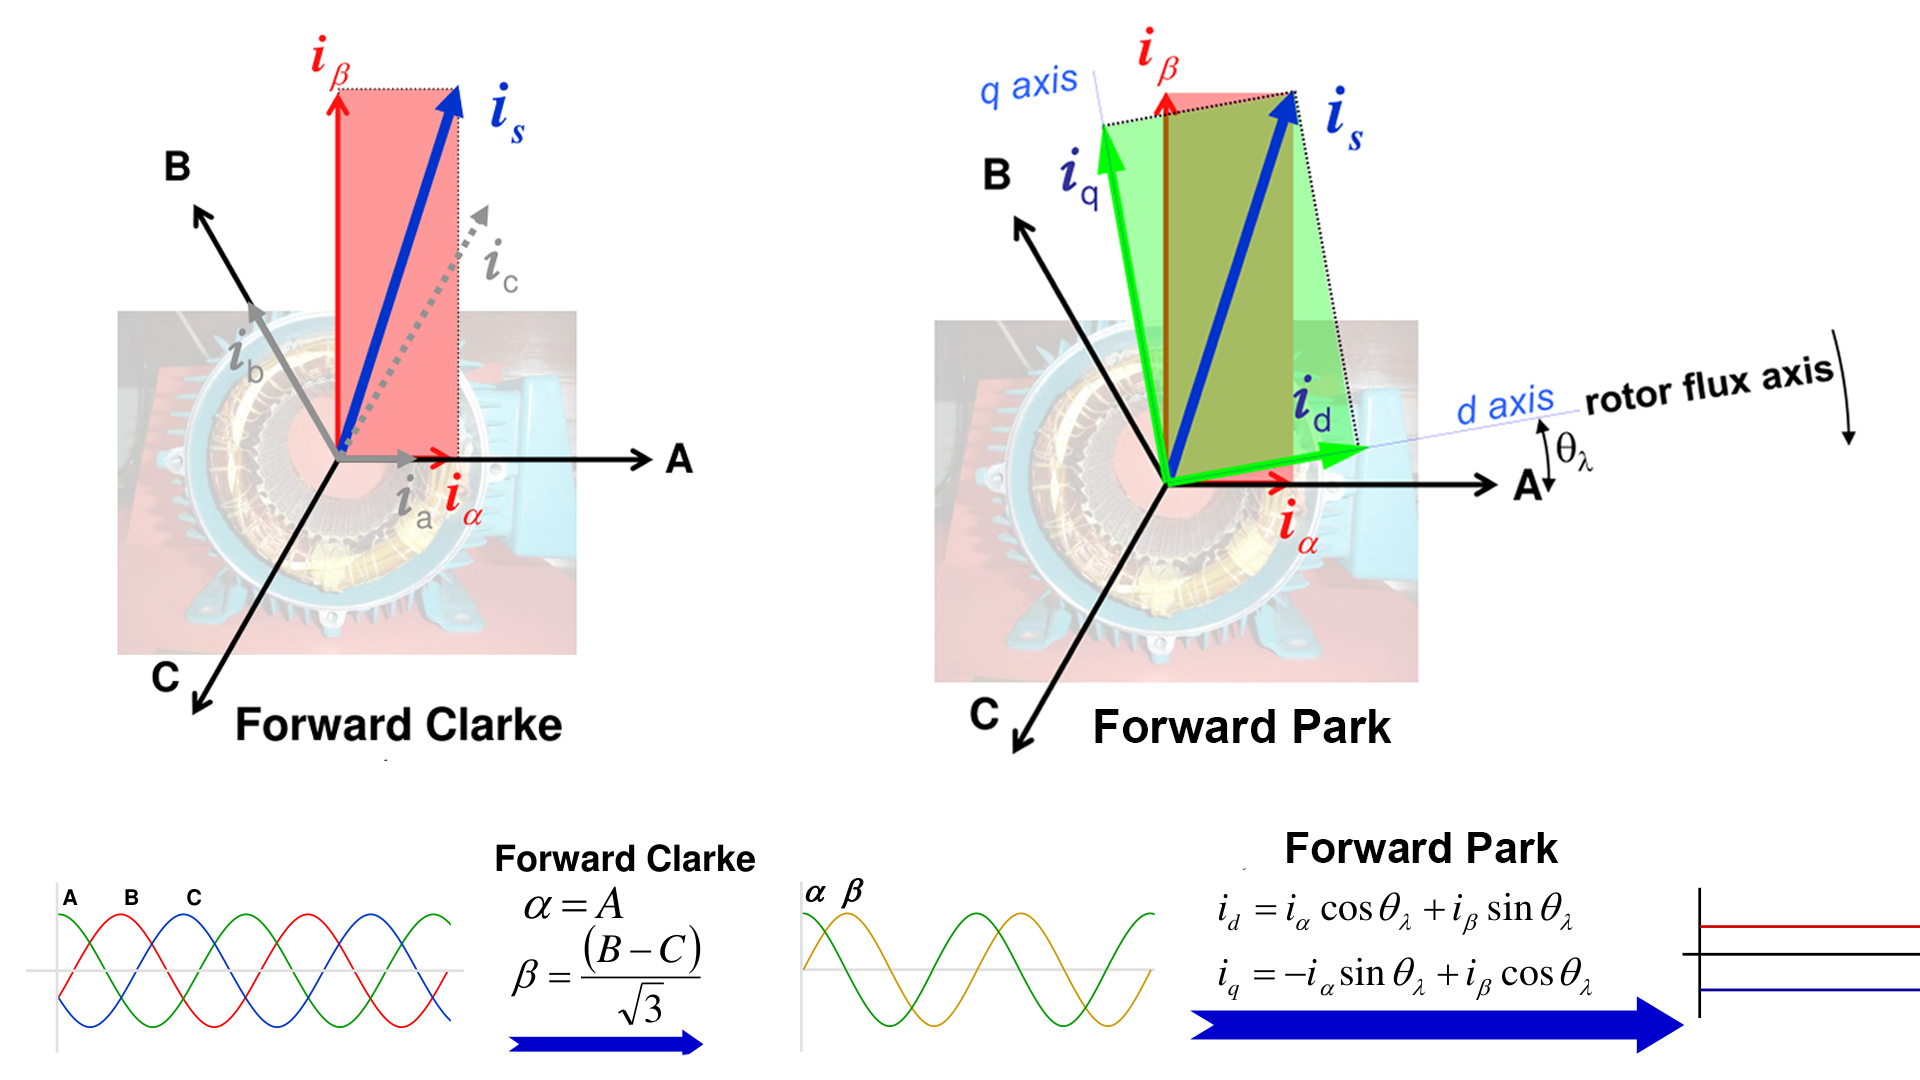
\includegraphics[width=4in]{sections/finalReview/coordianteTransforms.png}}
		\caption{Coordinate Transformations}
	\end{figure}
\end{frame}

\begin{frame}{Advantages of Field Oriented Control (FOC)}
	\begin{itemize}
		\item \textbf{Dynamic Response:} Faster and more accurate response to changes.
		\item \textbf{High torque:} FOC provides high torque at low speeds.
		\item \textbf{Efficiency:} Reduced energy consumption and increased performance.
		\item \textbf{Speed Control:} Precise and accurate control of motor's speed.
	\end{itemize}
\end{frame}




\begin{frame}{Hardware block diagram}
	\begin{figure}
		\centering

		\fbox{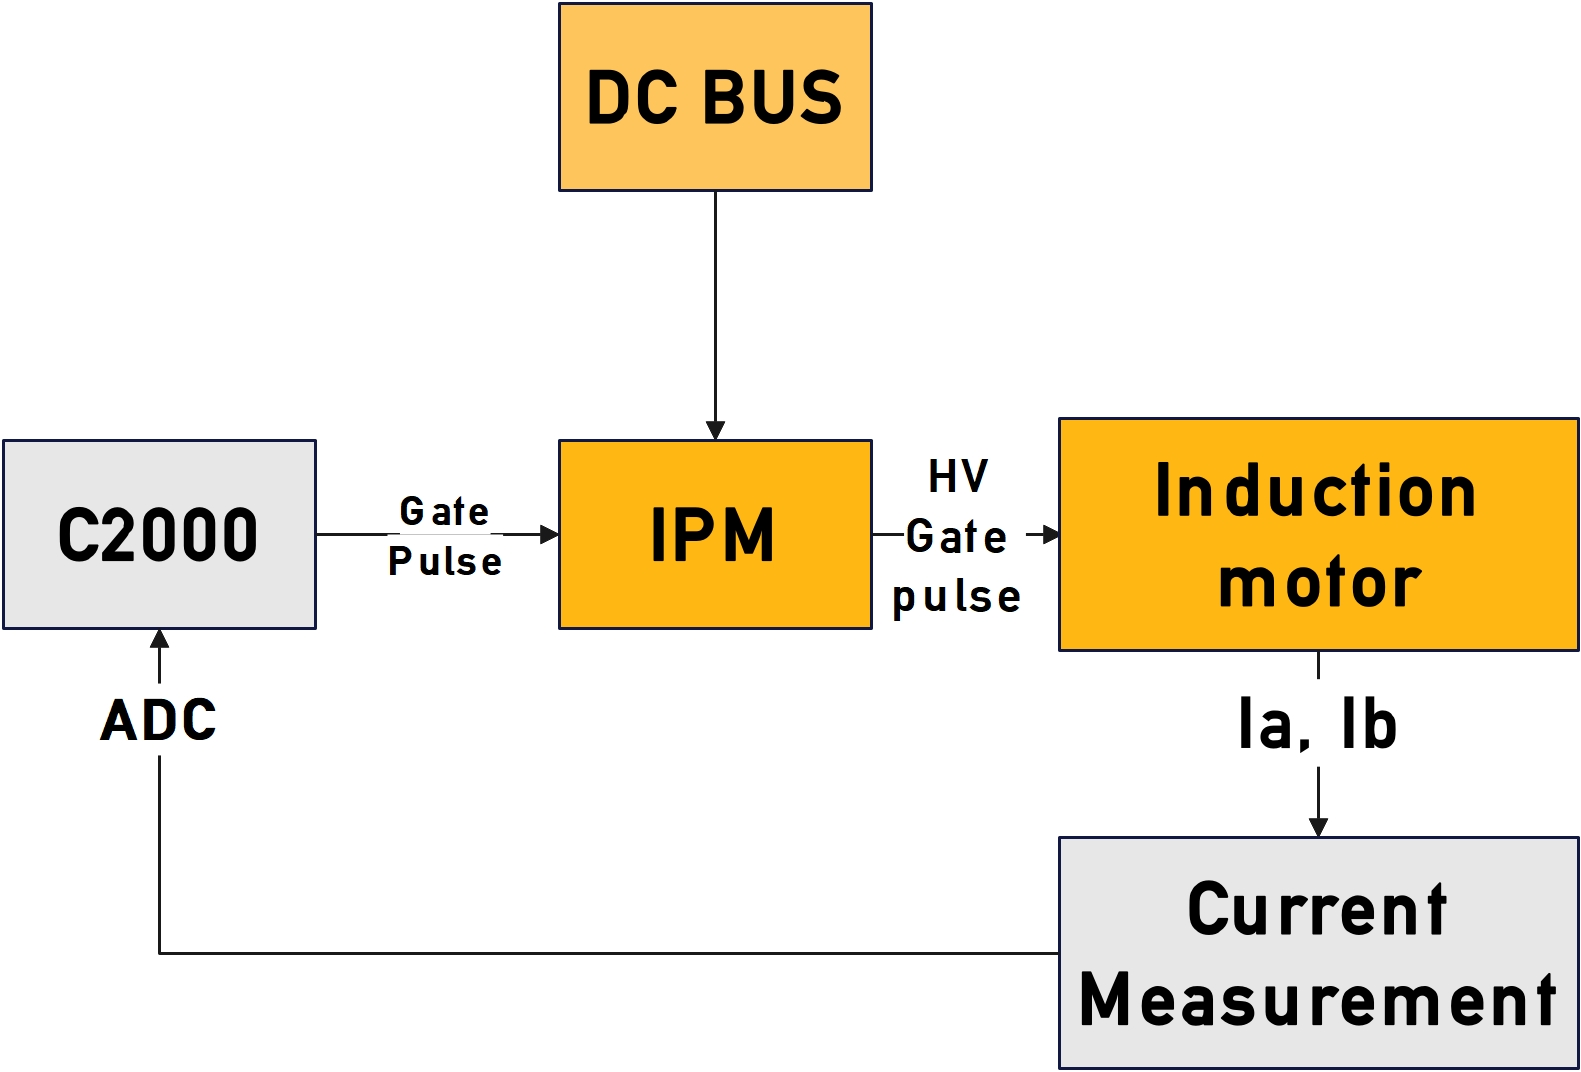
\includegraphics[width=4in]{sections/section4/images/SingleLineHardware.jpg}}

		\caption{Hardware block diagram}
	\end{figure}
\end{frame}


\begin{frame}{C2000 Features for Implementing Vector Control Algorithm}
	\begin{columns}
		\column{0.5\textwidth}
		\begin{minipage}[c]{\linewidth}
			\begin{figure}

				\centering
				\fbox{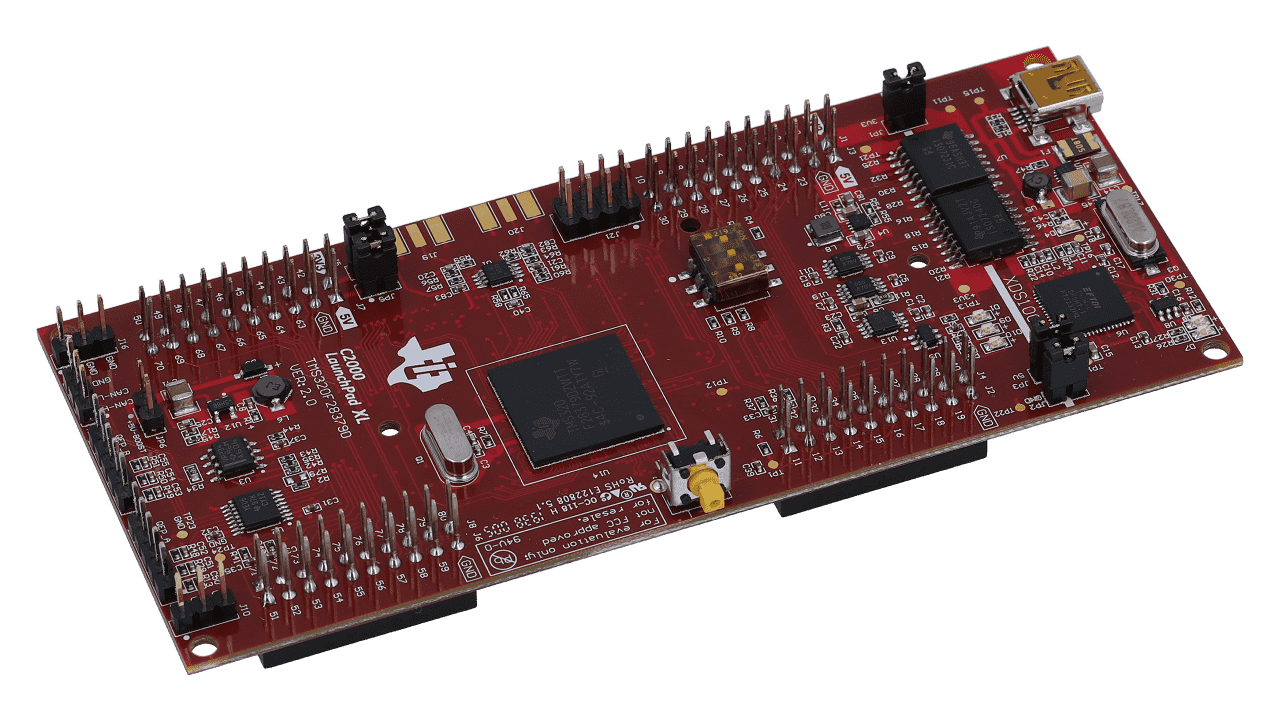
\includegraphics[width=2in]{sections/section4/images/f23879d/launchxl-f28379d-angled.png}}
				\caption{F28379D Launchpad}

			\end{figure}
		\end{minipage}
		\column{0.5\textwidth}
		\begin{itemize}
			\item 200 MHz C28x CPU
			\item Control Law Accelerator (CLA)
			\item 12-bit/16-bit ADCs
			\item Enhanced Pulse Width Modulators (ePWM)
		\end{itemize}
	\end{columns}
\end{frame}

\begin{frame}{Intelligent Power Module FSAM20SH60A}
	\begin{columns}
		\column{0.3\textwidth}
		\begin{figure}
			\centering
			\fbox{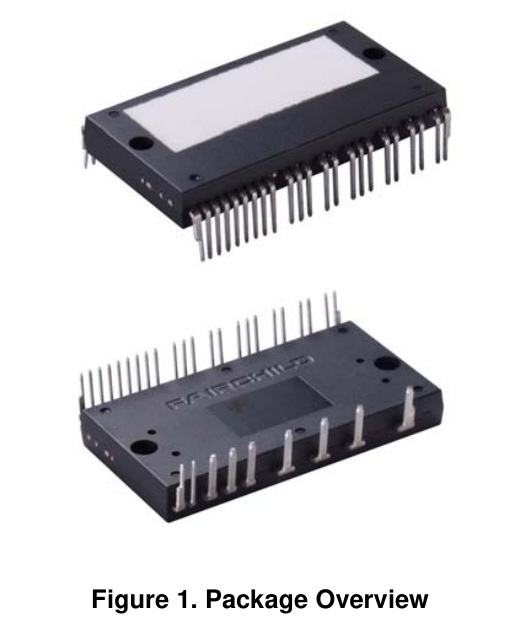
\includegraphics[width=1.3in]{sections/section4/images/IPM/ipm.png}}
			\caption{Intelligent Power Module FSAM20SH60A}
		\end{figure}
		\column{0.6\textwidth}
		\begin{itemize}
			\item \textbf{Compact Design:} Integrates power devices, drivers, and protection circuitry.
			\item \textbf{Enhanced Performance:} Optimized for high-speed switching.
			\item \textbf{Protection Features:} Includes built-in under-voltage lockout, over-temperature protection, and fault reporting, enhancing system reliability.
			\item \textbf{Ease of Use} Simplifies system design and reduces time-to-market compared to designing with discrete components.
		\end{itemize}
	\end{columns}
\end{frame}


% discrete inverter vs IPM 2 images side by side

\begin{frame}{Discrete inverter vs IPM}
	\begin{figure}
		\begin{tabular}{cc}
			\fbox{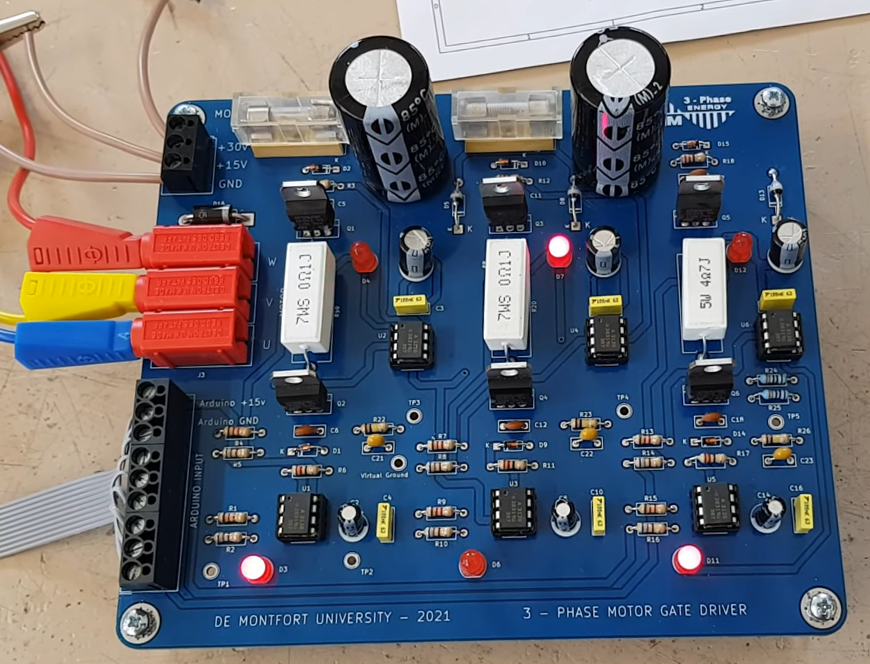
\includegraphics[width=1.9in]{sections/finalReview/discreteInverter.png}}
			 &
			\fbox{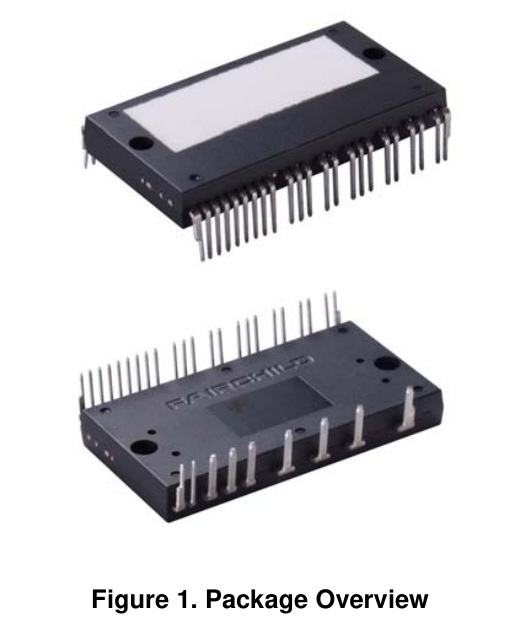
\includegraphics[width=1.2in]{sections/section4/images/IPM/ipm.png}} \\
			\small (a) Discrete Inverter
			 &
			\small (b) Intelligent Power Module (IPM)
		\end{tabular}
		\caption{Discrete Inverter vs Intelligent Power Module (IPM)}
	\end{figure}
\end{frame}



\begin{frame}{Induction Motor}
	\begin{tabular}{cc}
		\begin{minipage}[c]{0.4\textwidth}
			\centering
			\fbox{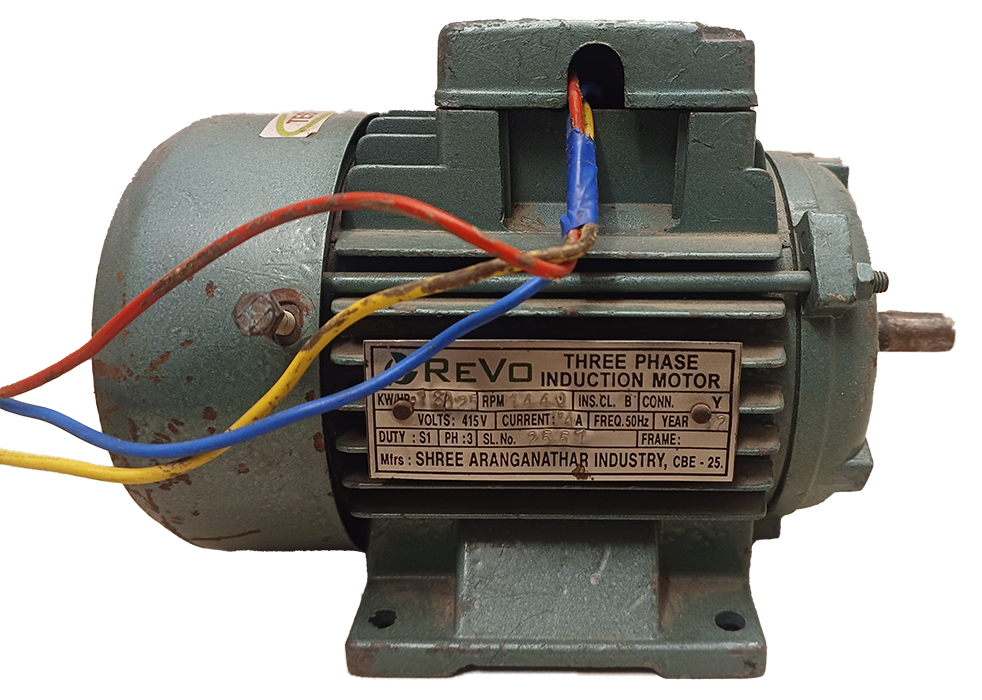
\includegraphics[width=1.8in]{sections/section4/images/inductionMotor/revo.png}}
			\captionof{figure}{Induction Motor}
		\end{minipage} &
		\begin{minipage}[c]{0.6\textwidth}
			\centering
			\begin{tabular}{|c|c|}
				\hline
				\textbf{Parameter} & \textbf{Value}  \\ \hline
				Power              & 0.25 Hp         \\ \hline
				Voltage            & 415 V (L-L) RMS \\ \hline
				Current            & 1.4 A           \\ \hline
				Frequency          & 50 Hz           \\ \hline
				Speed              & 1440 rpm        \\ \hline
				Phase              & 3               \\ \hline
			\end{tabular}
			\captionof{table}{Name-plate Details of Induction motor}
		\end{minipage}
	\end{tabular}
\end{frame}




% Slide 3: Block Diagram of the System
\begin{frame}{Block Diagram of the System}
	\begin{figure}
		\centering

		\fbox{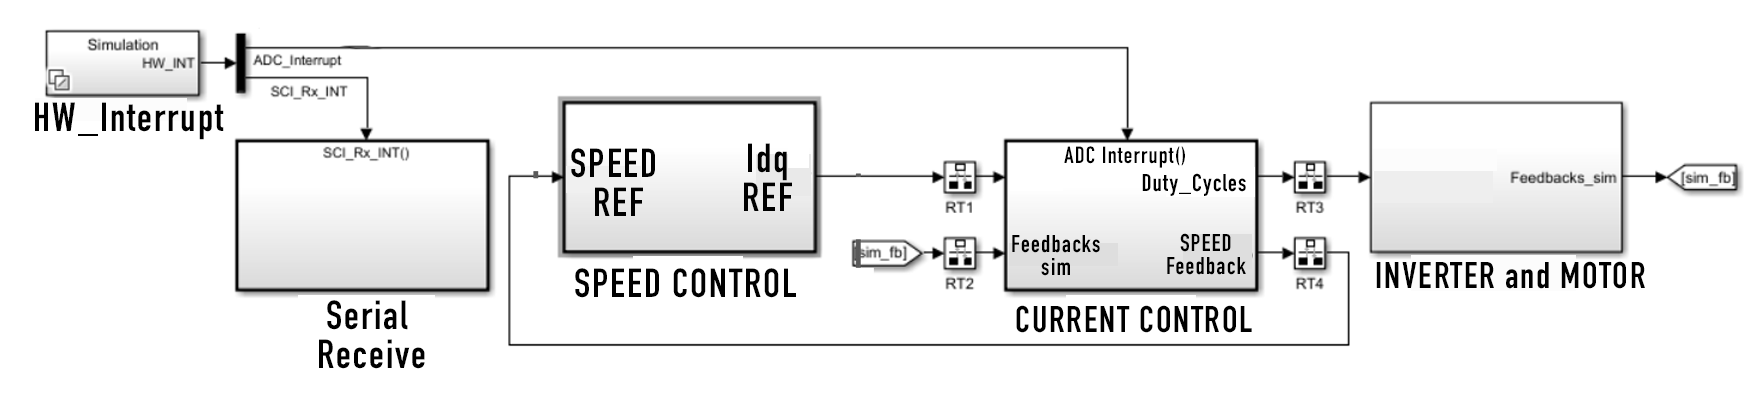
\includegraphics[width=4in]{sections/section3/images/simulation/blockDia.png}}
		\caption{Block Diagram of the System}
	\end{figure}
\end{frame}

% Slide 4: Speed Control Subsystem
\begin{frame}{Speed Control Subsystem}
	\vspace{-0.5cm} % adjust vertical space
	\begin{figure}
		\centering
		\fbox{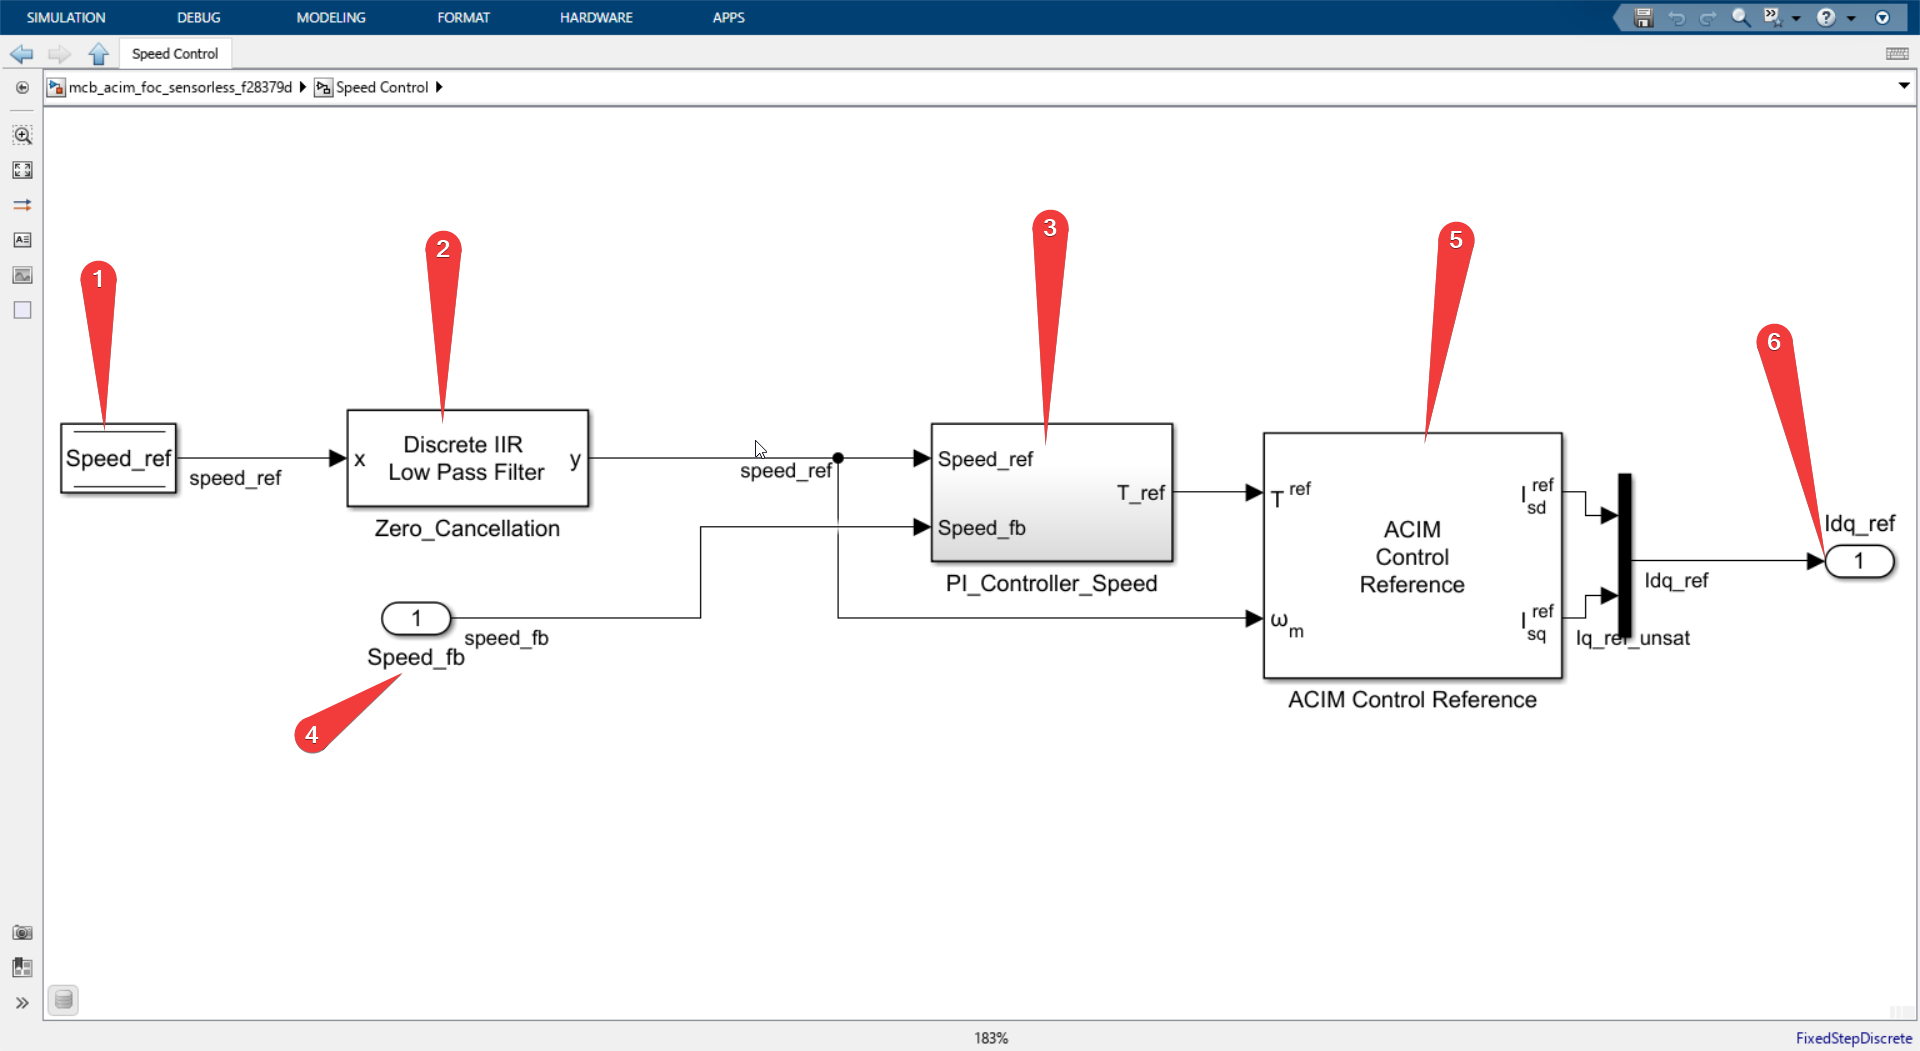
\includegraphics[width=4in]{sections/section3/images/simulation/speedControl/speedController.png}}
		\caption{Speed Control Subsystem}
	\end{figure}
	\vspace{-0.5cm} % adjust vertical space
	\begin{align}
		i_{d_0}    & = \frac{Z_{rd}}{L_m}                                                          \\
		i_{sq_req} & = \frac{T^{ref}}{3/2 \cdot P \cdot \left(\frac{L_m}{L_r}\right) \cdot i_{rd}}
	\end{align}
\end{frame}


% Slide 5: Current Measurement
\begin{frame}{Current Measurement}
	\begin{figure}
		\centering

		\fbox{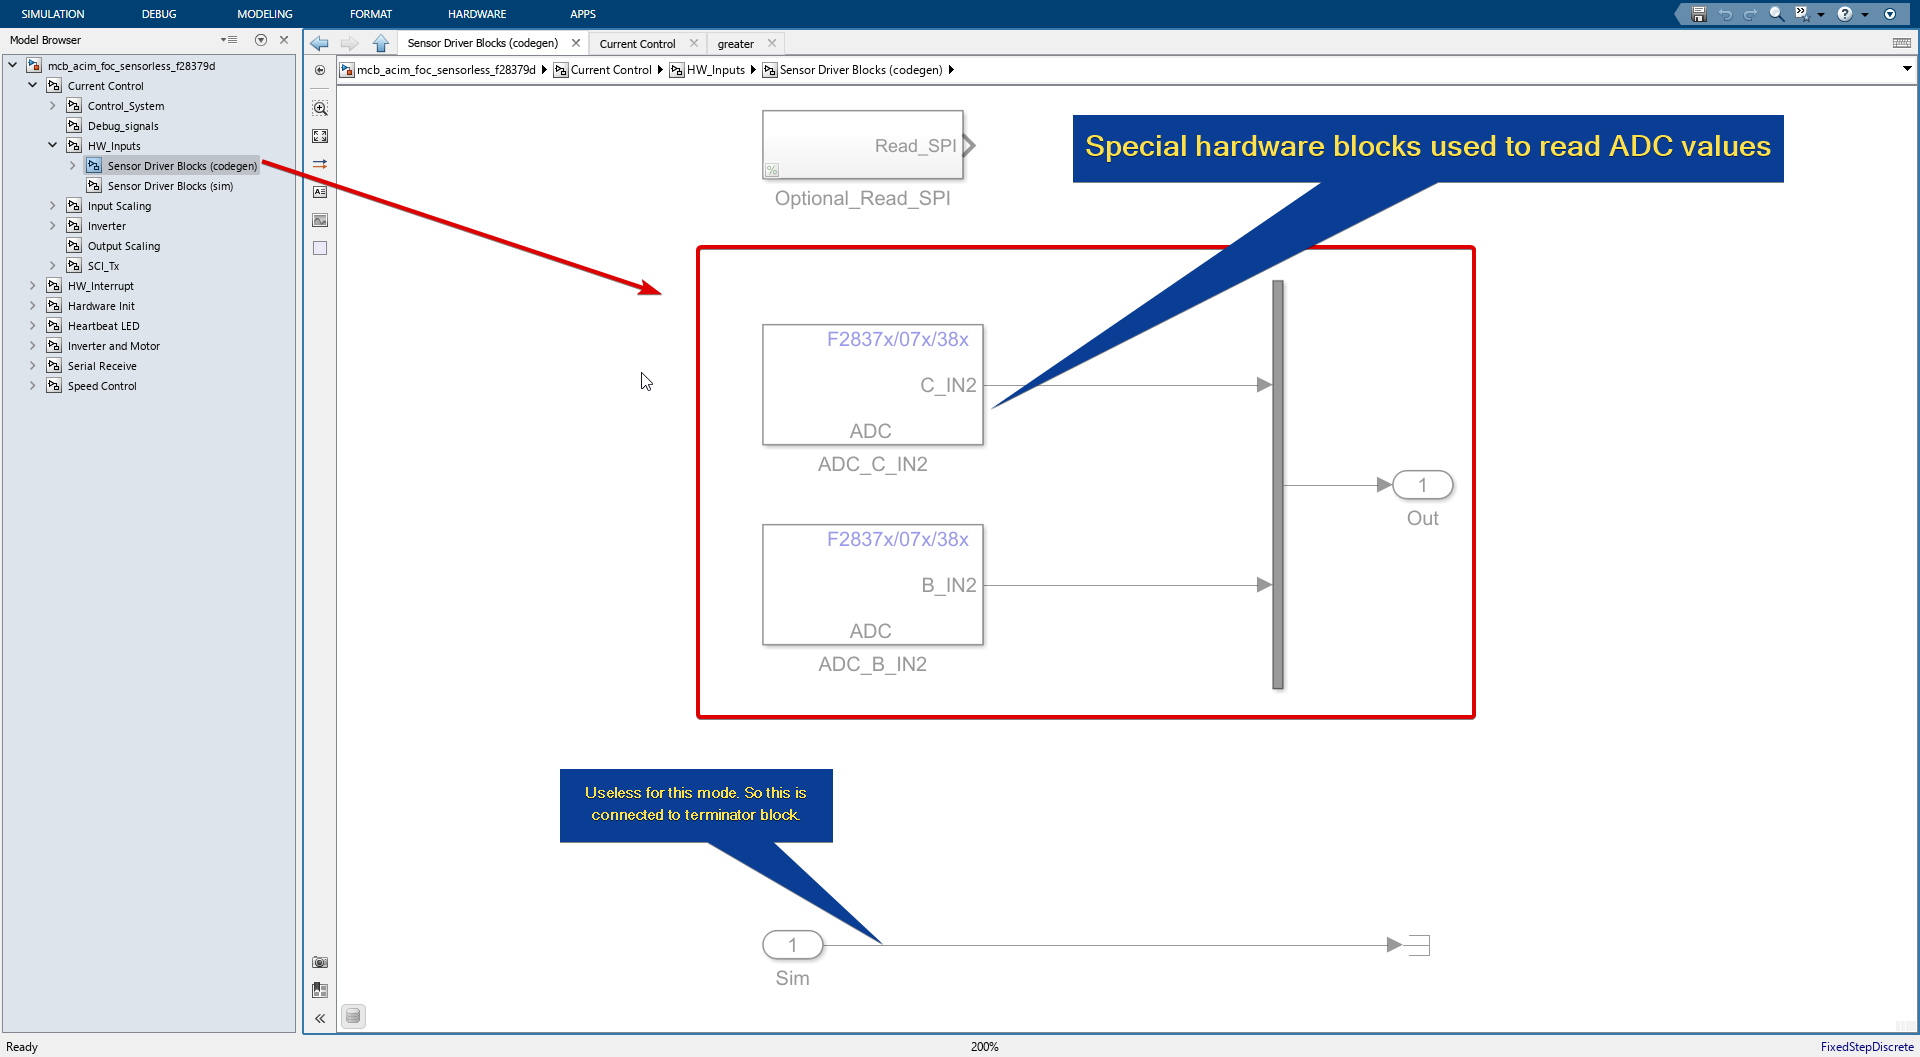
\includegraphics[width=4in]{sections/finalReview/adcBlock.png}}
		\caption{ADC block for reading current}
	\end{figure}
\end{frame}

\begin{frame}{Current Control System}
	\begin{figure}
		\centering

		\fbox{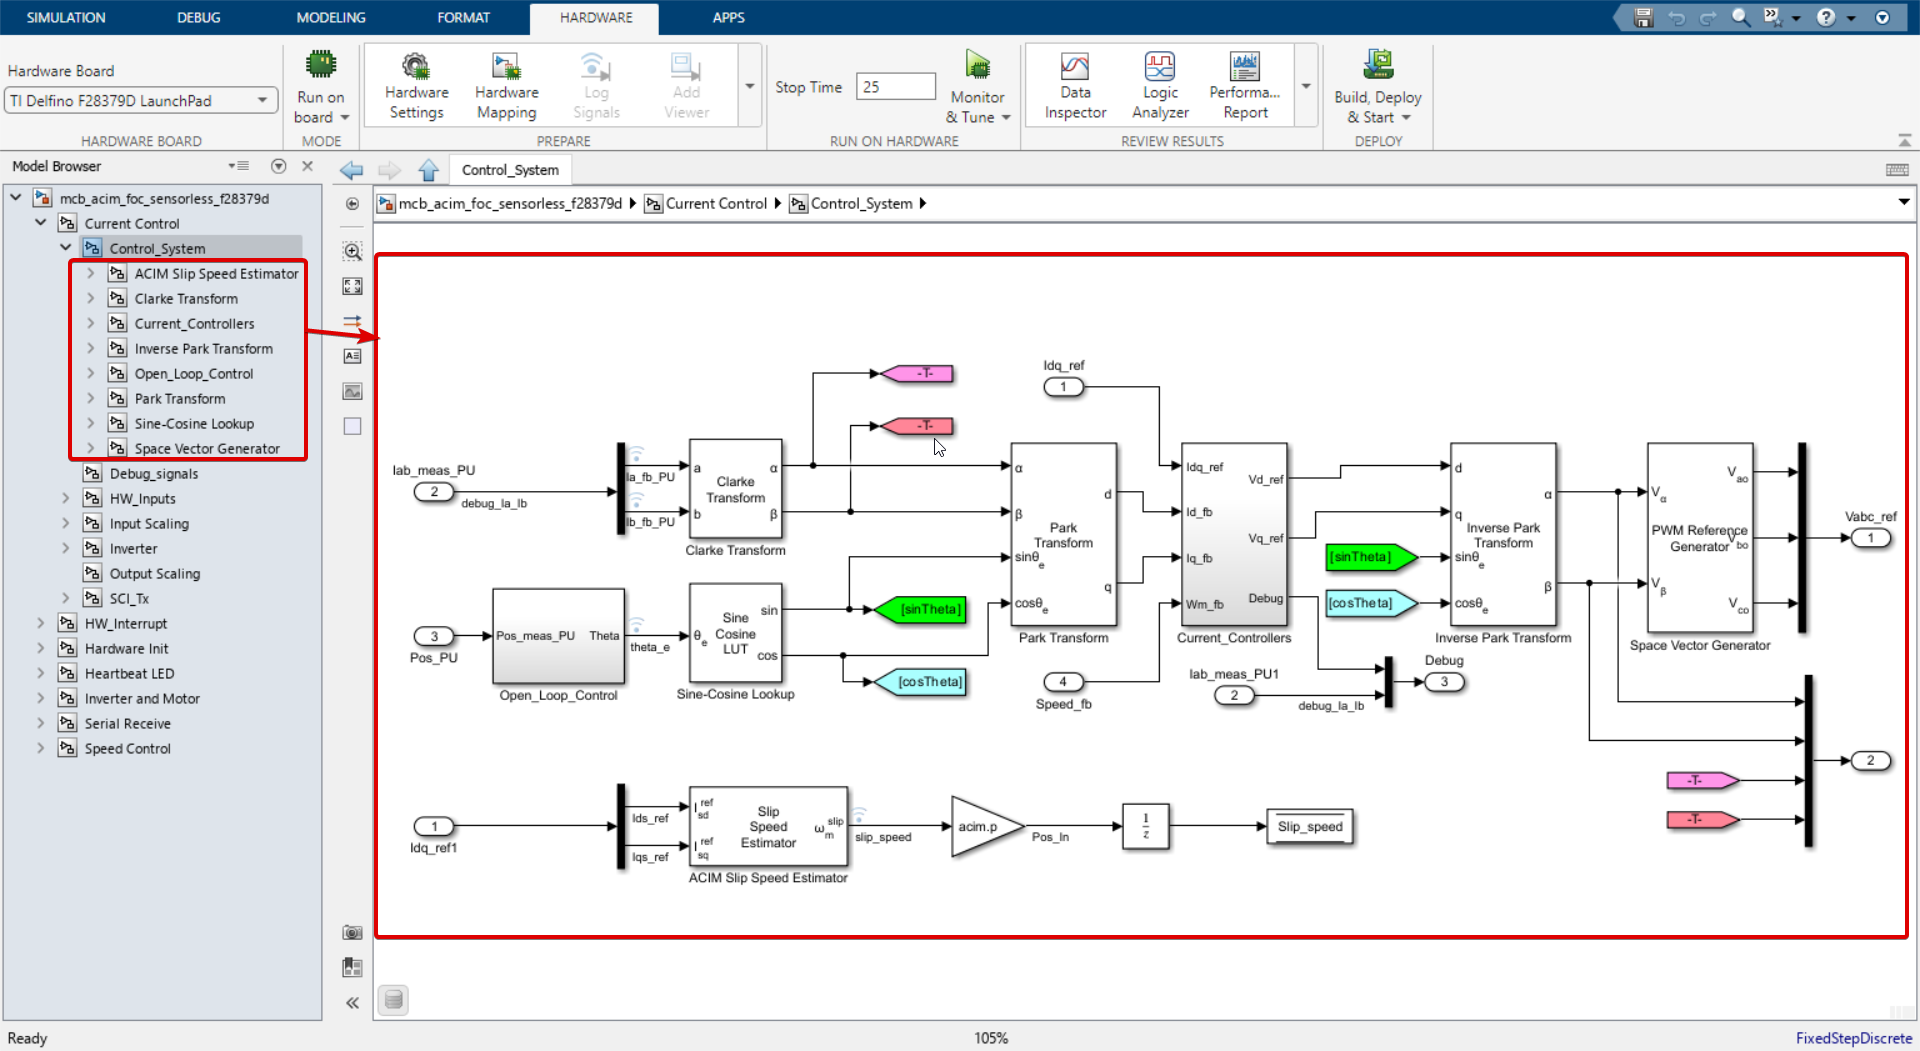
\includegraphics[width=4in]{sections/section3/images/simulation/currentControl/controlSystem.png}}
		\caption{Current Control System}
	\end{figure}
\end{frame}



\begin{frame}{Flux observer and Speed Estimation}
	\begin{columns}
		\column{0.4\textwidth}
		\begin{figure}
			\centering
			\fbox{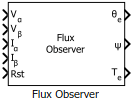
\includegraphics[width=1.2in]{sections/finalReview/fluxobserver.png}} % replace with your placeholder image
		\end{figure}
		\column{0.6\textwidth}
		\begin{equation*}
			\begin{gathered}
				\psi_a = \frac{L_r}{L_m} \left( \int (V_a - I_a R) dt - \sigma L_s I_a \right) \\
				\addlinespace
				\psi_b = \frac{L_r}{L_m} \left( \int (V_b - I_b R) dt - \sigma L_s I_b \right) \\
				\addlinespace
				\sigma = 1 - \frac{L_m^2}{L_r \cdot L_s} \\
				\addlinespace
				\theta_e = \tan^{-1} \frac{\psi_b}{\psi_a}
			\end{gathered}
		\end{equation*}
	\end{columns}
\end{frame}


% slip speed estimator

\begin{frame}{Slip Speed Estimator}
	\begin{columns}
		\column{0.4\textwidth}
		\begin{figure}
			\centering
			\fbox{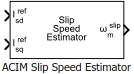
\includegraphics[width=1.2in]{sections/finalReview/slipspeed.png}} % replace with your placeholder image
		\end{figure}
		\column{0.6\textwidth}
		\begin{equation*}
			\begin{gathered}
				\tau_r = \left(\frac{L_r}{R_r}\right) \\[0.5em]
				\omega_\text{slip} = \left(\frac{1}{p}\right)\left(\frac{1}{\tau_r}\right)\left(\frac{i_\text{sq}^\text{ref}}{i_\text{sd}^\text{ref}}\right)
				\omega_e = \omega_r + \omega_{e_\text{slip}} \\[0.5em]
			\end{gathered}
		\end{equation*}
	\end{columns}
\end{frame}

% Slide 6: Position and Speed Estimation
\begin{frame}{Position and Speed Estimation}
	\begin{figure}
		\centering

		\fbox{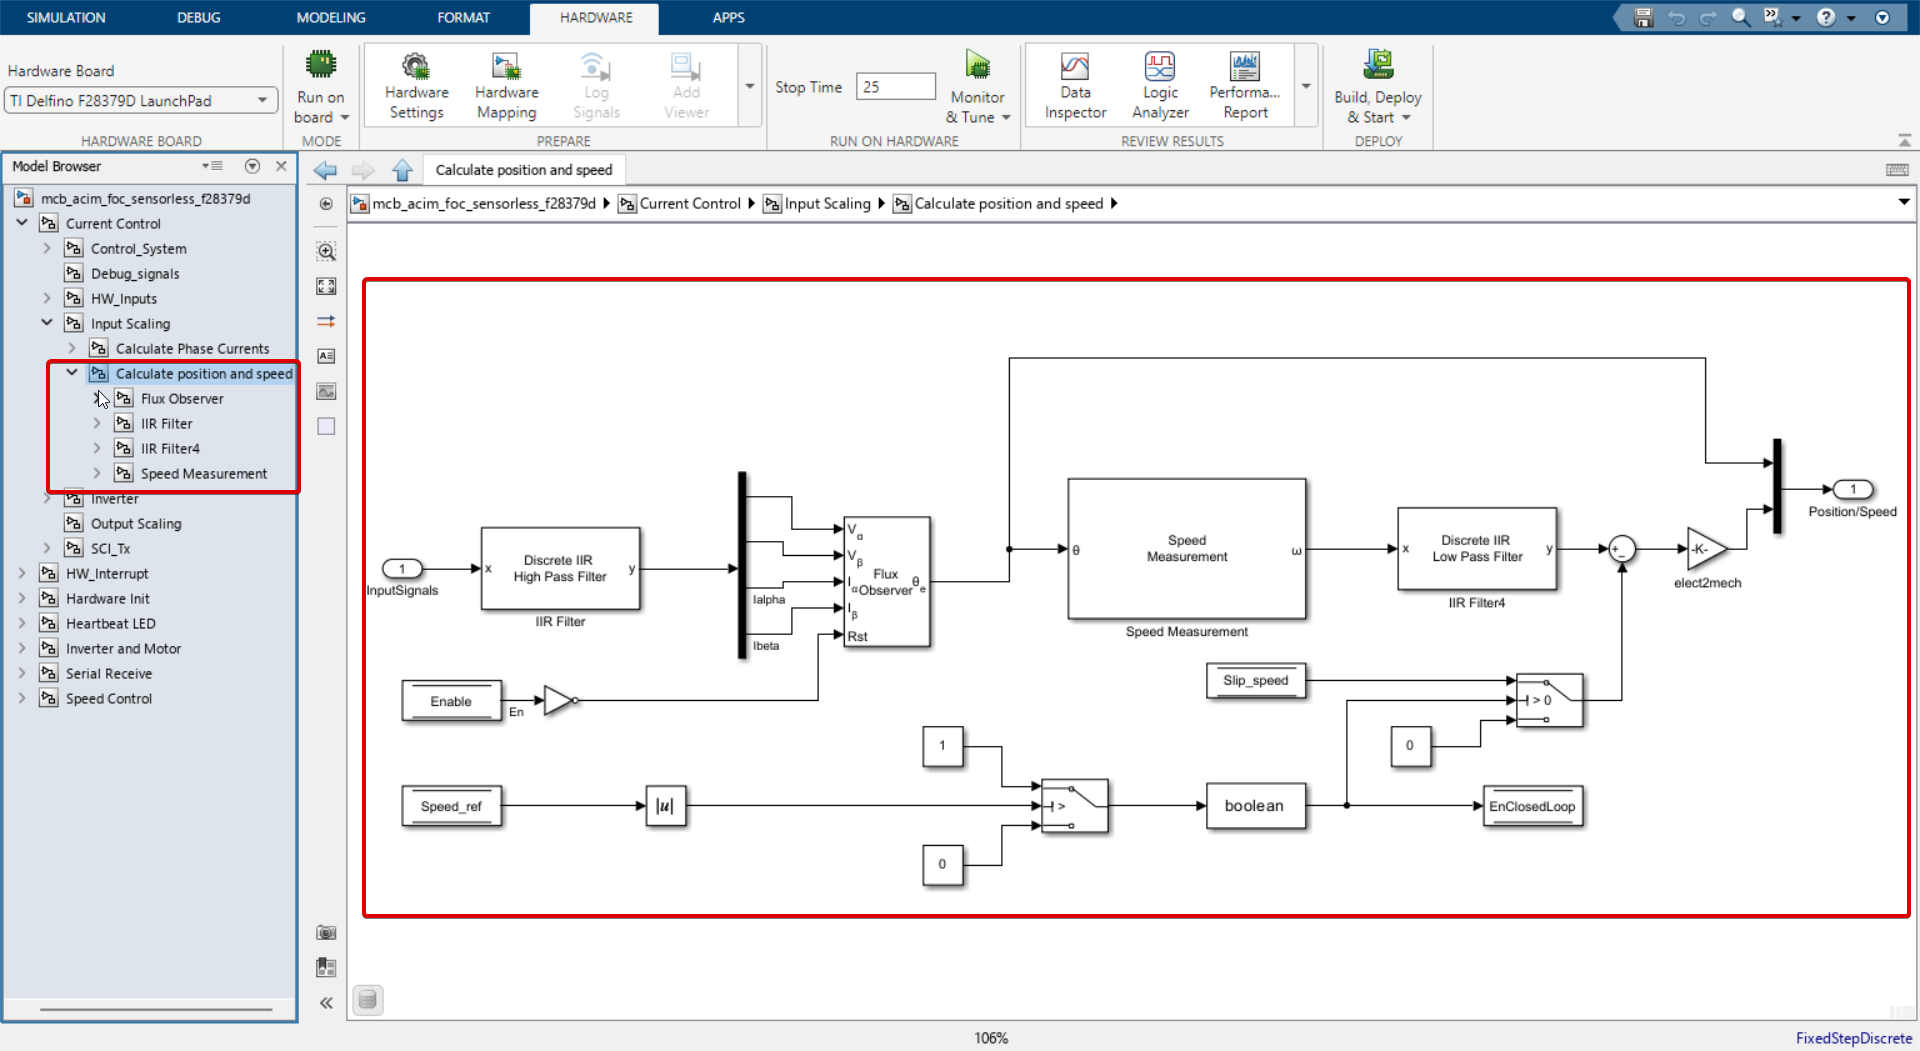
\includegraphics[width=4in]{sections/section3/images/simulation/inputScaling/fluxObserver.png}}
		\caption{Position and Speed Estimation}
	\end{figure}
\end{frame}


% Slide 7: Current Control System
\begin{frame}{Current Control System}
	\begin{figure}
		\centering

		\fbox{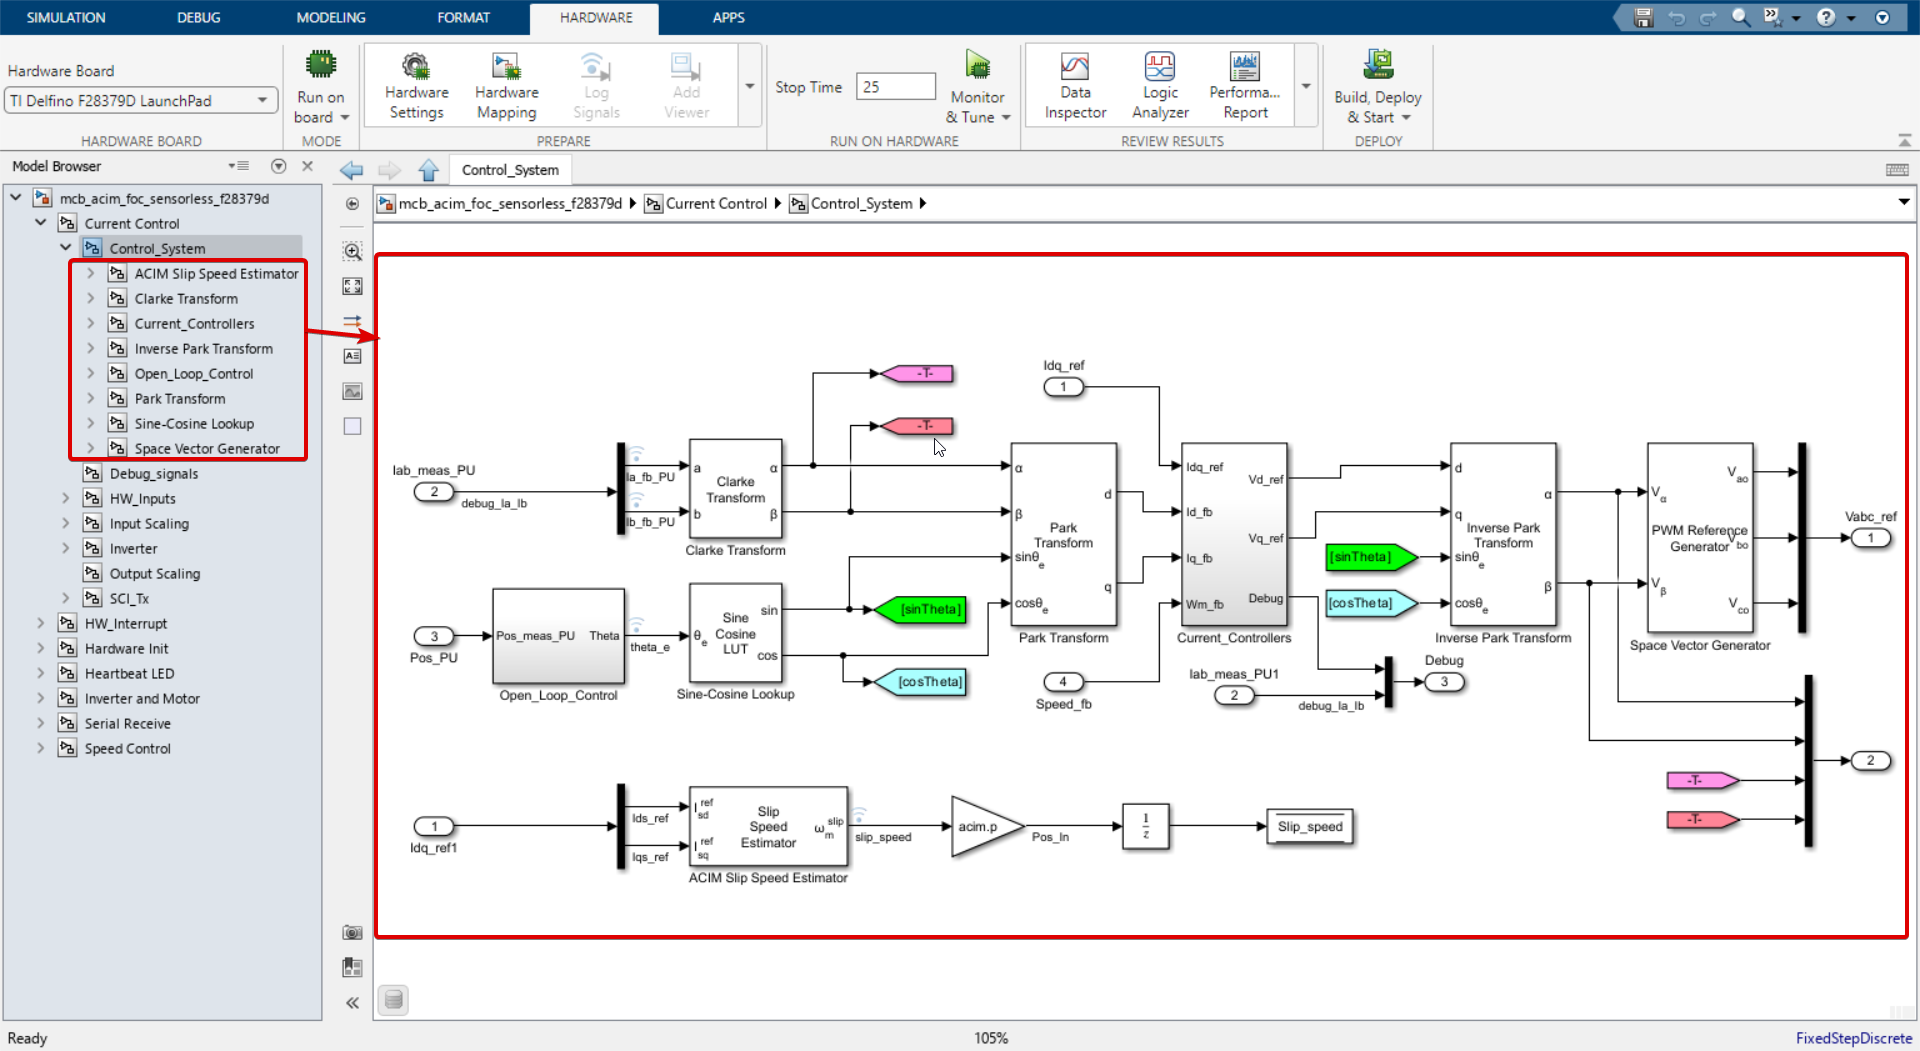
\includegraphics[width=4in]{sections/section3/images/simulation/currentControl/controlSystem.png}}
		\caption{Current Control System}
	\end{figure}
\end{frame}



\begin{frame}{ACIM required data}
	\begin{columns}
		\column{0.3\textwidth}
		\begin{figure}
			\centering
			\fbox{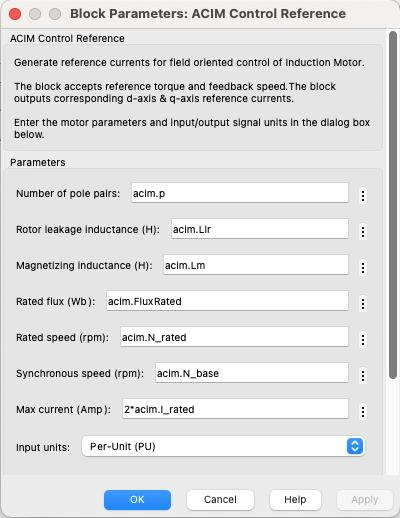
\includegraphics[width=1.3in]{sections/finalReview/dlgCurrentRef.jpg}}
			\caption{Current Reference}
		\end{figure}
		\column{0.3\textwidth}
		\begin{figure}
			\centering
			\fbox{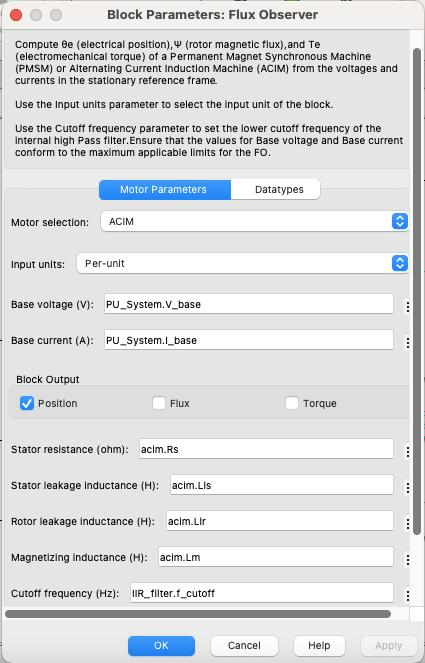
\includegraphics[width=1.2in]{sections/finalReview/dlgFlux.jpg}}
			\caption{Flux observer}
		\end{figure}
		\column{0.3\textwidth}
		\begin{figure}
			\centering
			\fbox{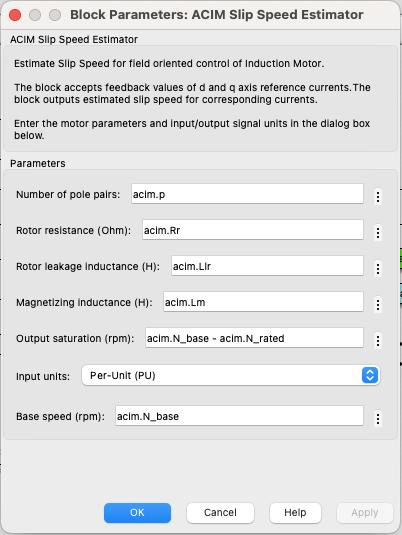
\includegraphics[width=1.5in]{sections/finalReview/dlgSlip.jpg}}
			\caption{Slip speed estimator}
		\end{figure}

	\end{columns}
\end{frame}

\begin{frame}{ACIM Parameter Estimation: No-Load Test}
	\begin{columns}
		\column{0.5\textwidth}
		\begin{figure}
			\centering
			\fbox{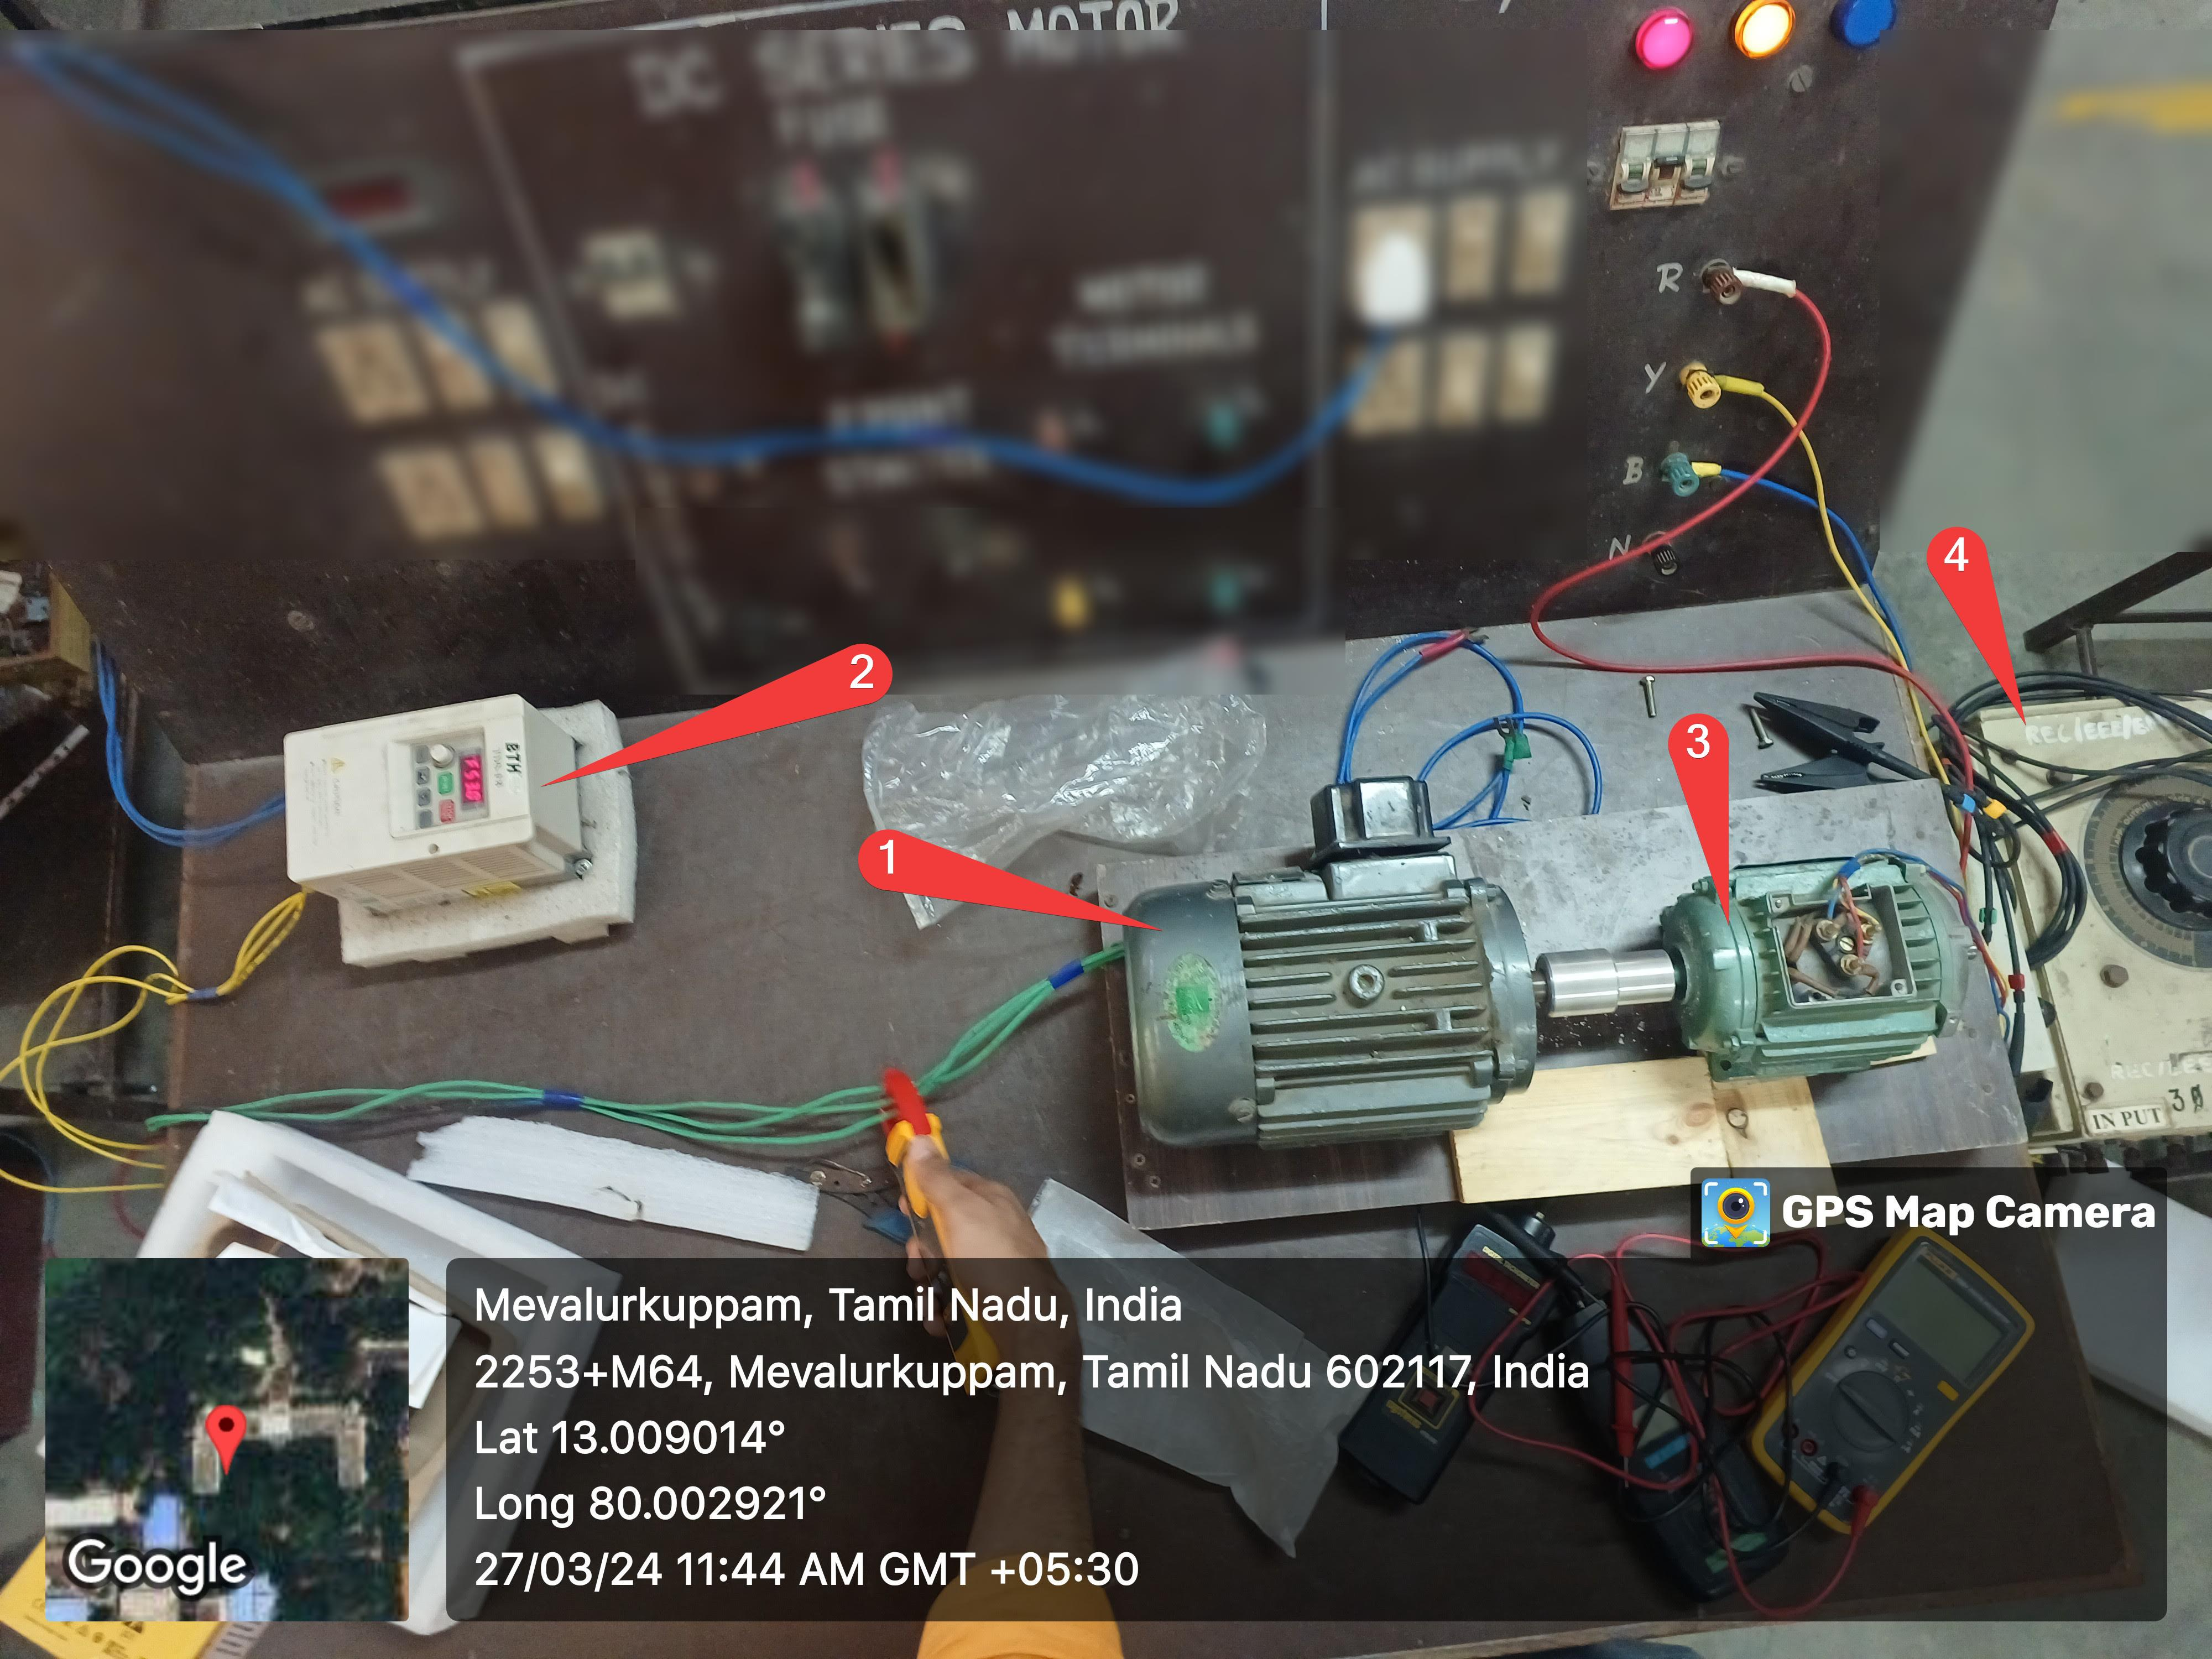
\includegraphics[width=2.2in]{sections/section5/images/ParamEstim/SetupNoload.jpg}}
			\caption{No-load test setup}
		\end{figure}
		\begin{itemize}
			\item Slip speed is made zero.
		\end{itemize}
		\column{0.5\textwidth}
		\begin{figure}
			\centering
			\fbox{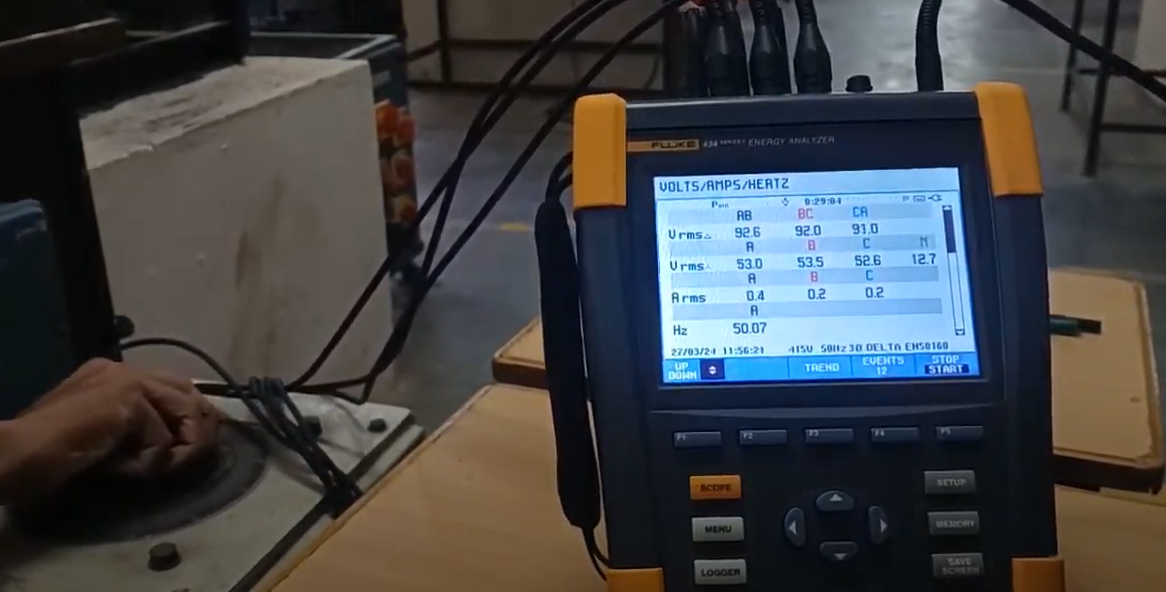
\includegraphics[width=2.2in]{sections/section5/images/ParamEstim/FlukeVoltAmpHertz.png}}
			\caption{Fluke 434 power analyzer}
		\end{figure}
	\end{columns}
\end{frame}

% Slide: No-load and Blocked Rotor Test Circuits
\begin{frame}{ACIM Parameter Estimation: Test Circuits}
	\begin{columns}
		\column{0.5\textwidth}
		\begin{figure}
			\centering
			\fbox{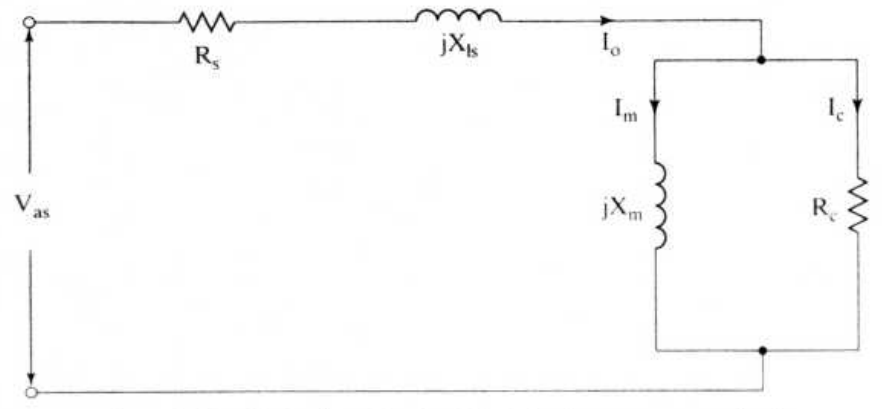
\includegraphics[width=2in]{sections/section5/images/ParamEstim/noloadCircuitKrish.png}}
			\caption{No-load test circuit}
		\end{figure}
		\column{0.5\textwidth}
		\begin{figure}
			\centering
			\fbox{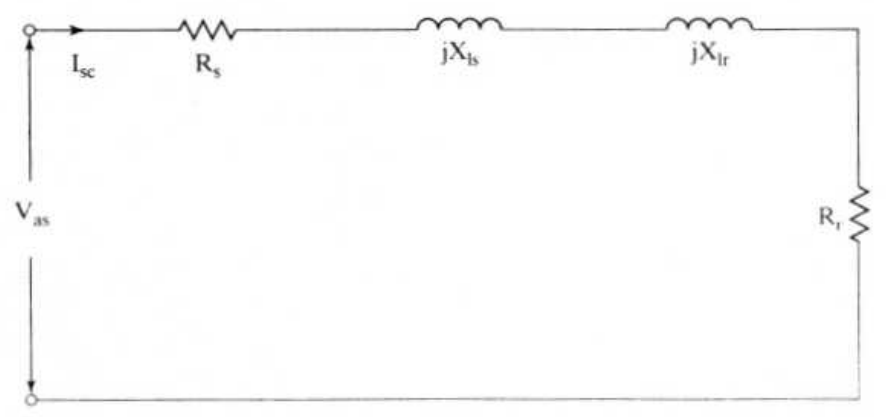
\includegraphics[width=2in]{sections/section5/images/ParamEstim/blockedCircuitKrish.png}}
			\caption{Blocked rotor test circuit}
		\end{figure}
	\end{columns}
\end{frame}
% ACIM formuls

\begin{frame}{ACIM Parameter Estimation Formulas}
	\begin{columns}[T] % Align columns at the top

		\begin{column}{0.48\textwidth} % Adjust column widths as needed

			\textbf{No-Load Test:}

			\begin{align*}
				\cos \phi_0 & = \frac{P_i}{V_\text{as}I_0}             \\
				I_m         & = I_0 \sin \phi_0                        \\
				I_c         & = I_0 \cos \phi_0                        \\
				L_m         & = \frac{V_\text{as}}{2\pi f_\text{i}I_m} \\
				R_c         & = \frac{V_\text{as}}{I_c}
			\end{align*}

		\end{column}

		\begin{column}{0.48\textwidth}

			\textbf{Blocked Rotor Test:}

			\begin{align*}
				\cos \phi_\text{sc} & = \frac{P_\text{sc}}{V_\text{sc}I_\text{sc}} \\
				Z_\text{sc}         & = \frac{V_\text{sc}}{I_\text{sc}}            \\
				R_r                 & = Z_\text{sc} \cos \phi_\text{sc} - R_s      \\
				X_\text{eq}         & = Z_\text{sc} \sin \phi_\text{sc}            \\
				X_\text{eq}         & = X_\text{ls} + X_\text{lr}
			\end{align*}

		\end{column}

	\end{columns}
\end{frame}



\begin{frame}{ACIM Parameter Estimation Results}
	\begin{columns}
		\column{0.5\textwidth}
		\begin{figure}
			\centering
			\fbox{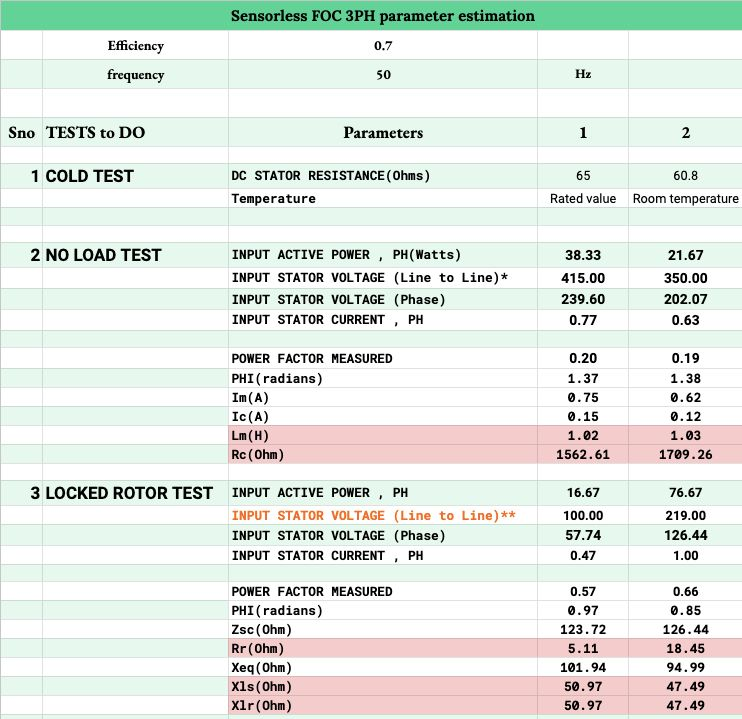
\includegraphics[width=2.2in]{sections/ppt/acim.jpg}}
			\caption{ACIM Parameter Estimation Results}
		\end{figure}
		\column{0.5\textwidth}
		\scalebox{0.8}{
			\begin{tabular}{|l|l|}
				\hline
				\multicolumn{2}{|c|}{No-Load Test} \\
				\hline
				Parameter             & Value      \\
				\hline
				POWER FACTOR MEASURED & 0.20       \\
				PHI (radians)         & 1.37       \\
				Im (A)                & 0.75       \\
				Ic (A)                & 0.15       \\
				Lm (H)                & 1.02       \\
				Rc (Ohm)              & 1562.61    \\
				\hline
				\multicolumn{2}{|c|}{Blocked Test} \\
				\hline
				Parameter             & Value      \\
				\hline
				POWER FACTOR MEASURED & 0.57       \\
				PHI (radians)         & 0.97       \\
				Zsc (Ohm)             & 123.72     \\
				Rr (Ohm)              & 5.11       \\
				Xeq (Ohm)             & 101.94     \\
				Xls (Ohm)             & 50.97      \\
				Xlr (Ohm)             & 50.97      \\
				\hline
			\end{tabular}
		}
	\end{columns}
\end{frame}




\begin{frame}{Rotor Load Angle}
	\begin{figure}
		\centering
		\fbox{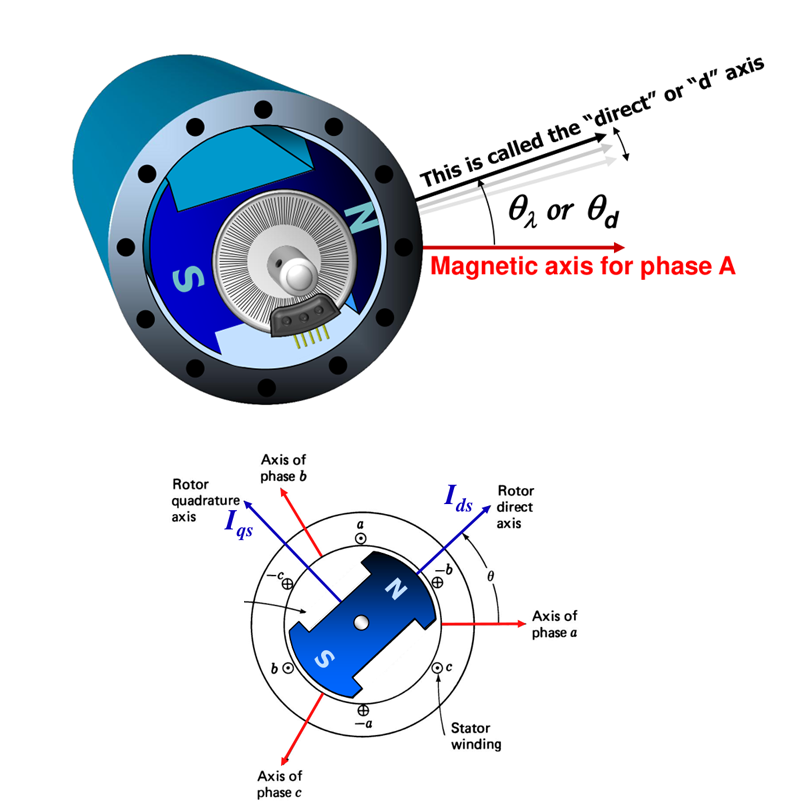
\includegraphics[width=2.5in]{sections/finalReview/rotorFlux.png}}
		\caption{Rotor Load Angle}
	\end{figure}
\end{frame}





% Slide 8: Speed Response
\begin{frame}{Speed Response}
	\begin{figure}
		\centering

		\fbox{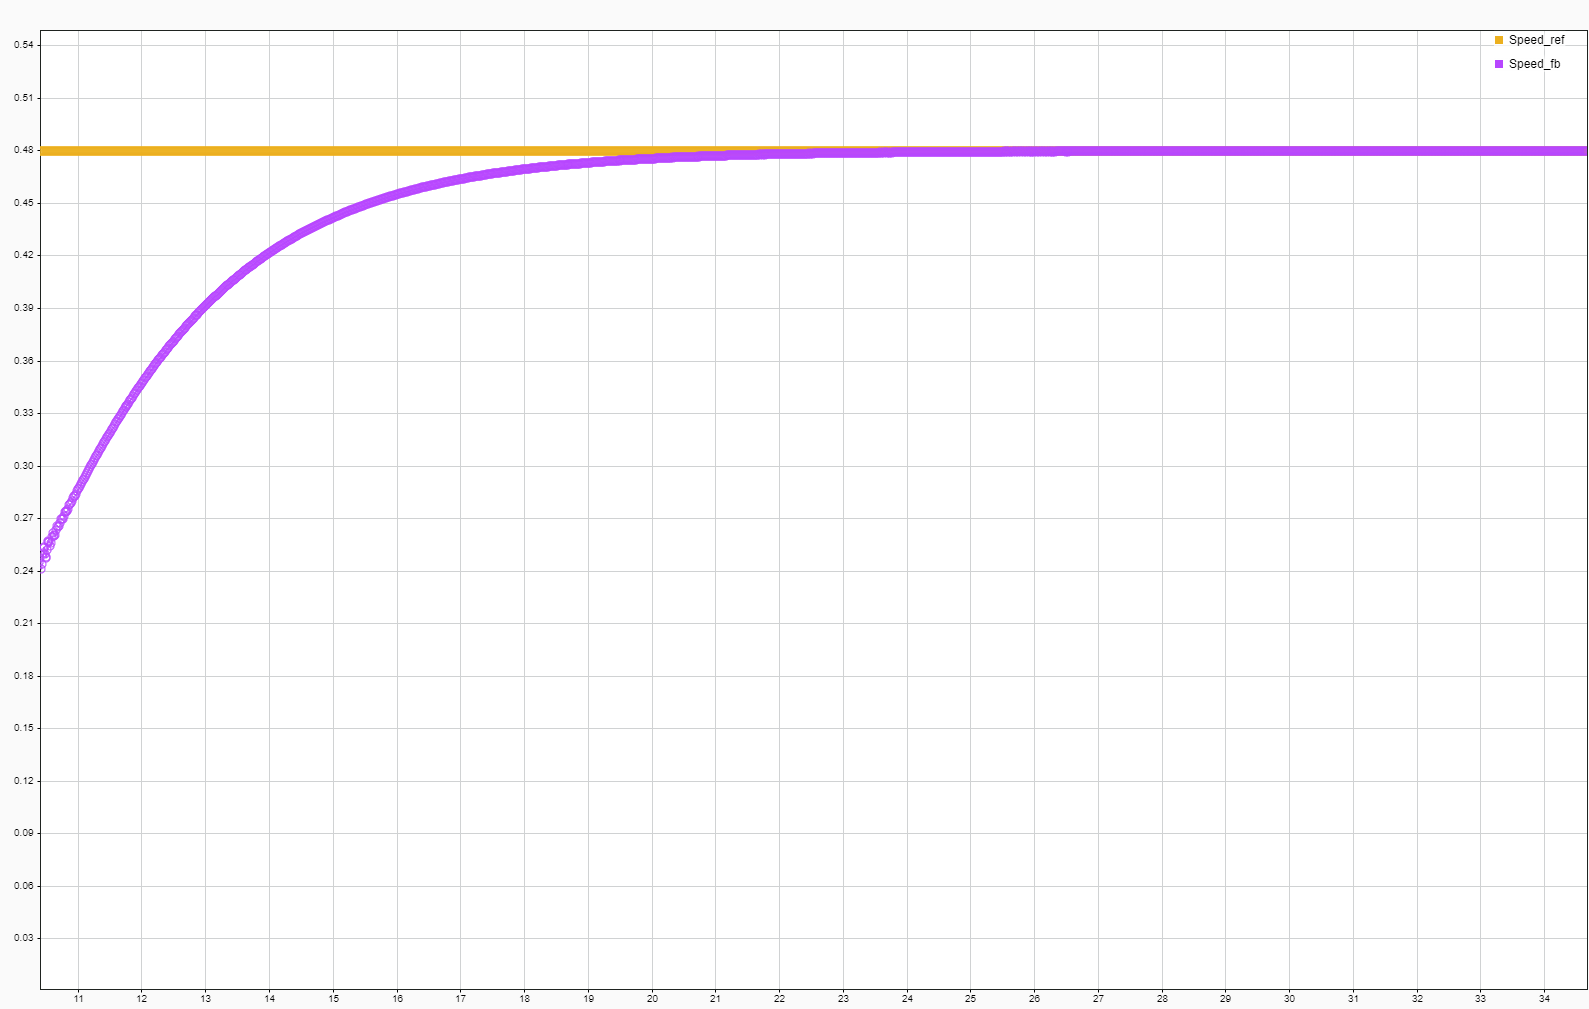
\includegraphics[width=4in]{sections/section3/images/simulationResutls/SpeedTrackingNoCursor.png}}
		\caption{Speed Response}
	\end{figure}
\end{frame}


\begin{frame}{Ia and Ib Feedback/Measured Currents}
	\begin{figure}
		\centering

		\fbox{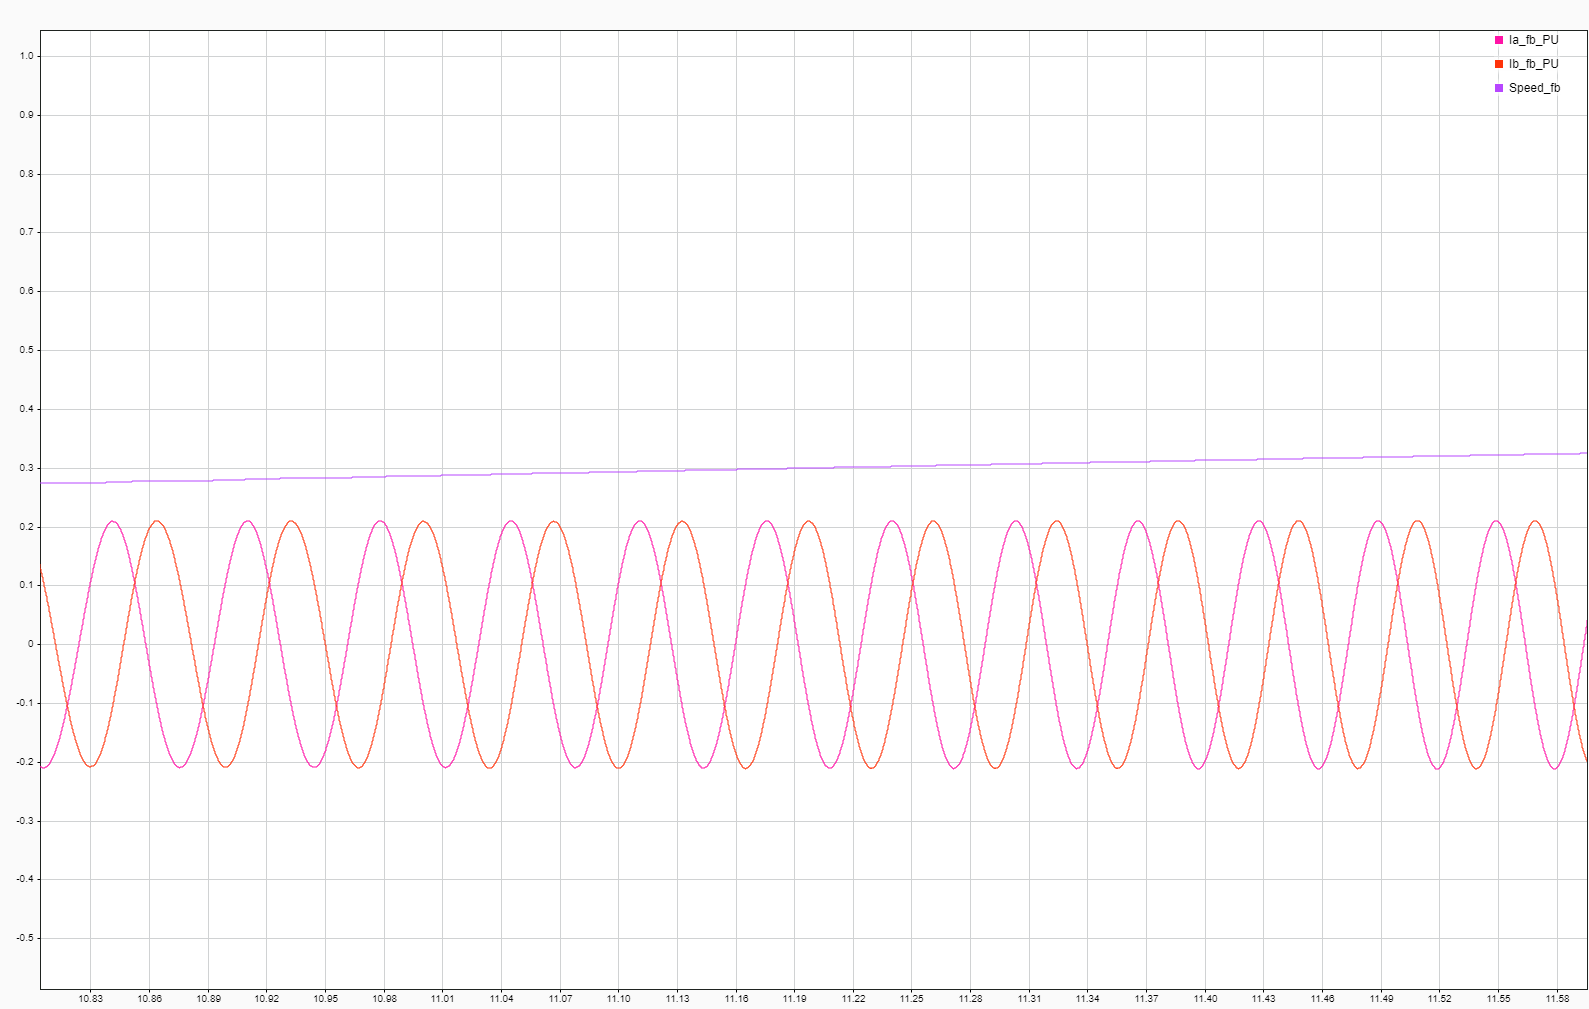
\includegraphics[width=4in]{sections/section3/images/simulationResutls/Ia_Ib_fb.png}}
		\caption{Ia and Ib Feedback/Measured Currents}
	\end{figure}
\end{frame}


% Slide 13: Iq Reference and Feedback Currents (Torque producing current)
\begin{frame}{Iq Reference and Feedback Currents (Torque producing current)}
	\begin{figure}
		\centering

		\fbox{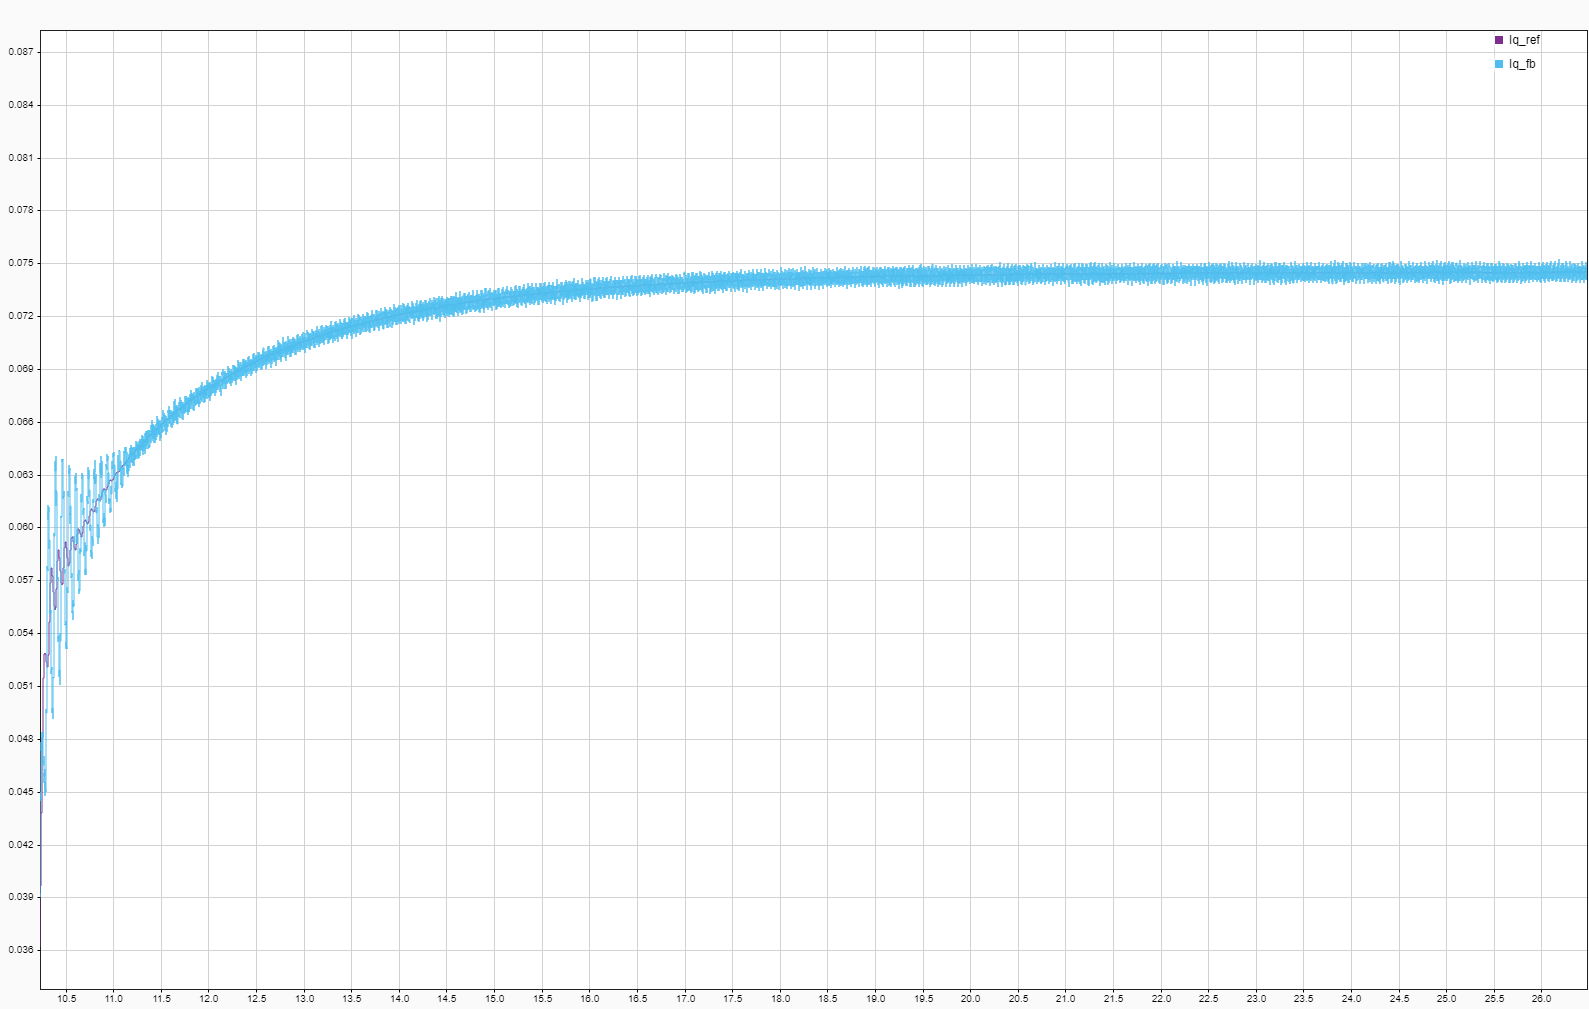
\includegraphics[width=4in]{sections/section3/images/simulationResutls/Iq_ref_fb.png}}

	\end{figure}
\end{frame}

% Slide 14: Id Reference and Feedback Currents (Magnetizing current)
\begin{frame}{Id Reference and Feedback Currents (Magnetizing current)}
	\begin{figure}
		\centering

		\fbox{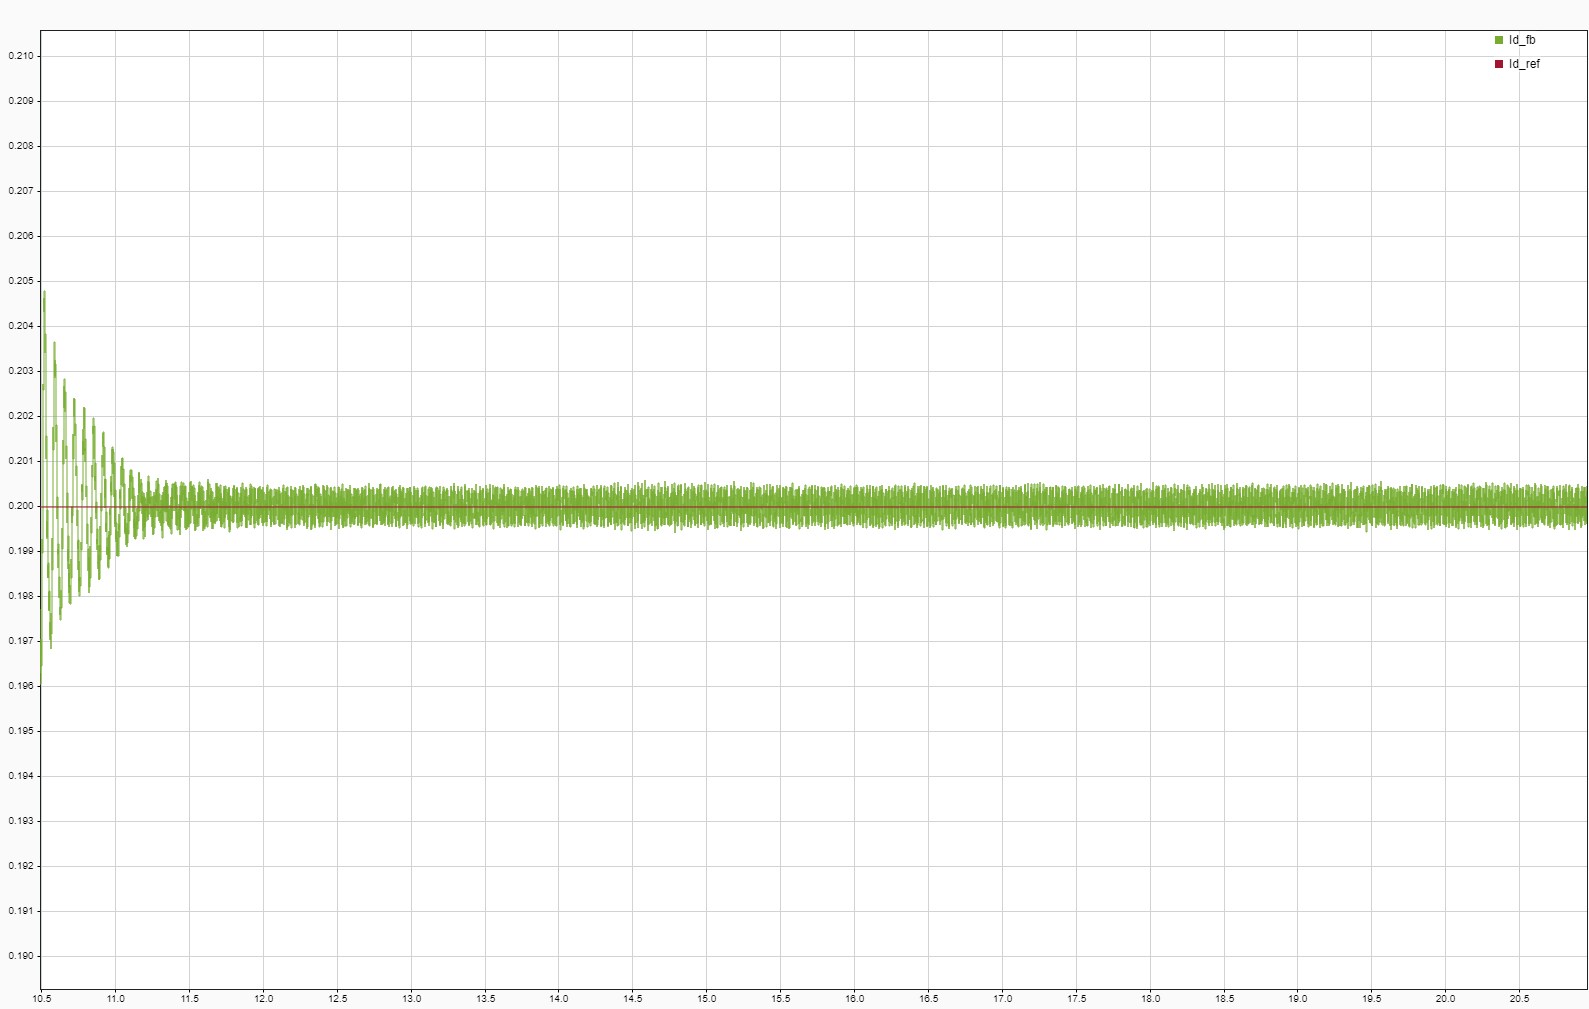
\includegraphics[width=4in]{sections/section3/images/simulationResutls/Id_ref_fb.png}}

	\end{figure}
\end{frame}



\begin{frame}{MATLAB/Simulink Implementation}
	\begin{figure}
		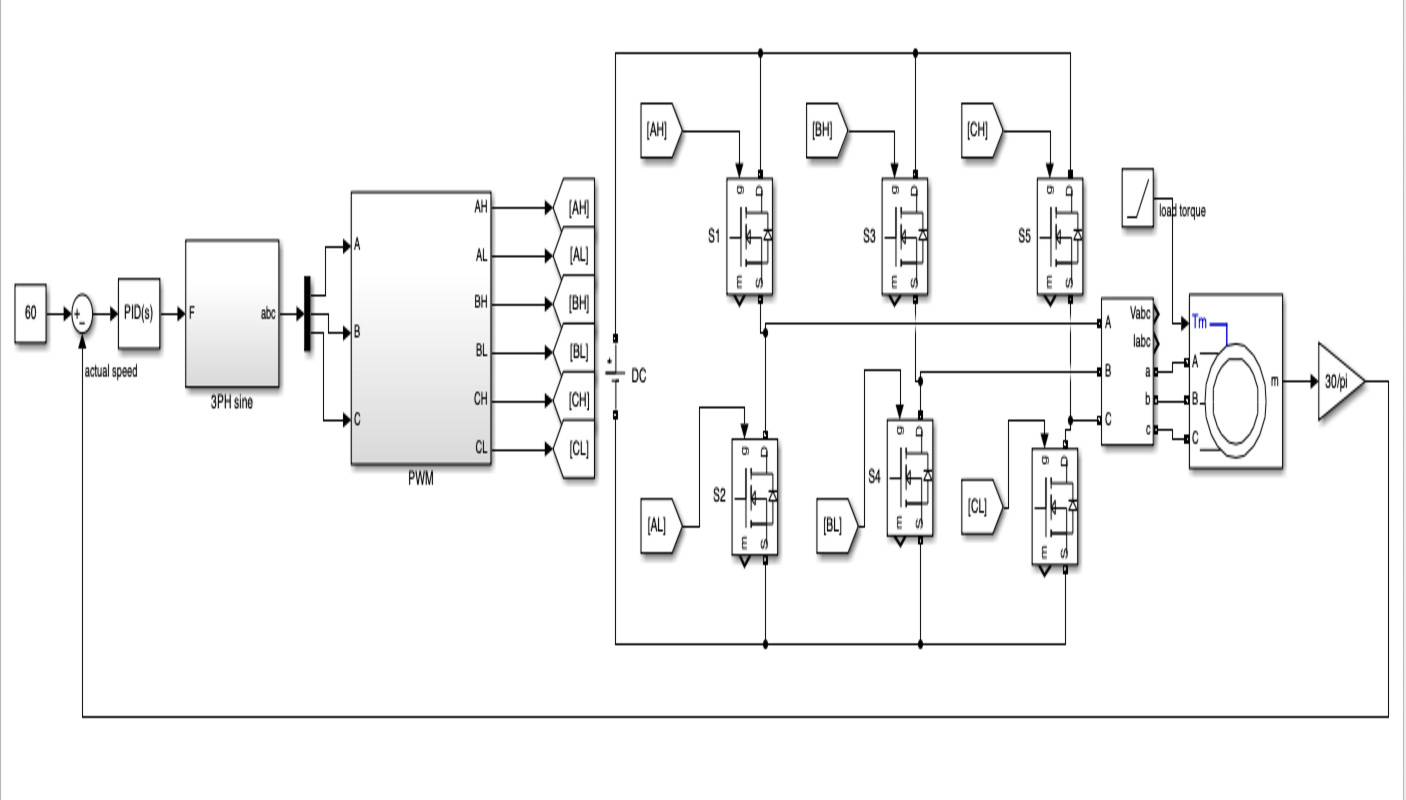
\includegraphics[width=3in]{conference/vfSimulation.png} % Replace with your V/f control Simulink image
		\caption{V/f Control Simulink Diagram}
	\end{figure}
\end{frame}


\begin{frame}{Performance Comparison: Torque Response}
	\begin{figure}
		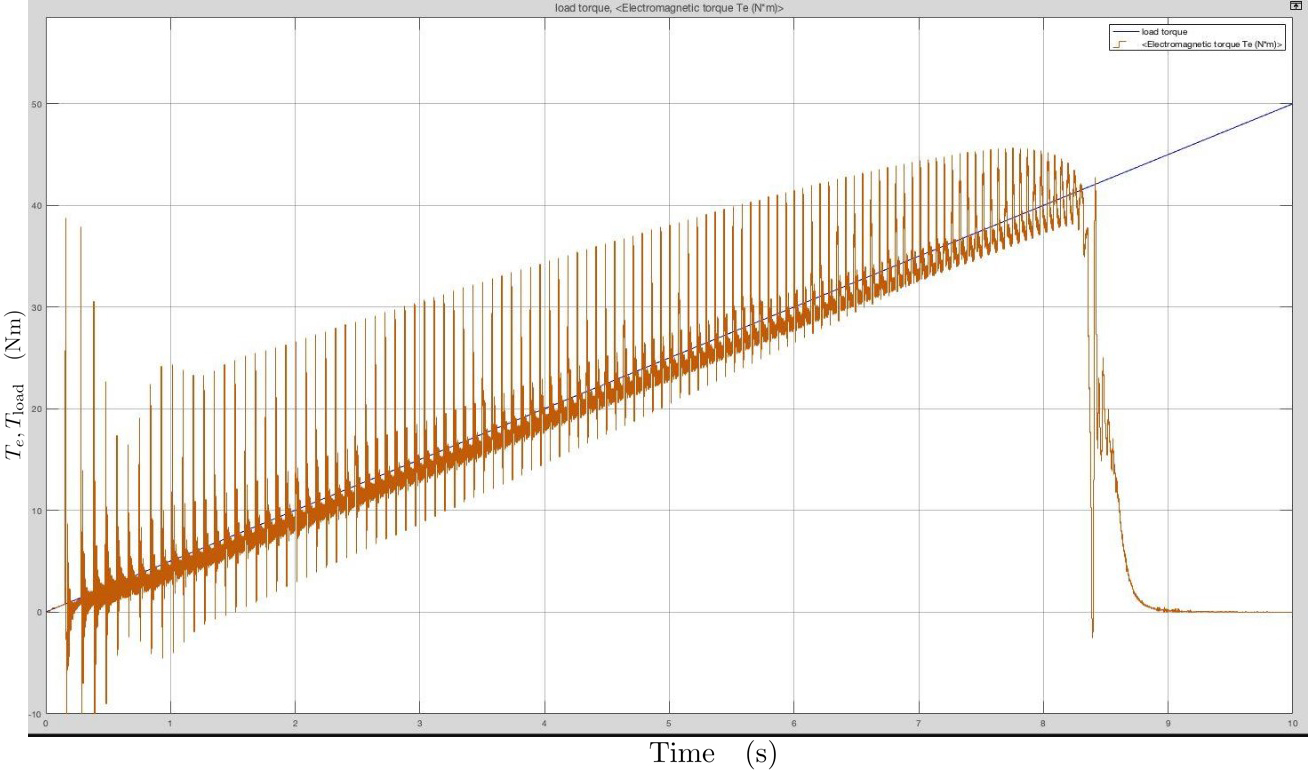
\includegraphics[width=4in]{conference/60rpmTorque.jpeg} % Replace with your torque response comparison graph
		\caption{Torque Response of V/F with ramp input}
	\end{figure}
\end{frame}

\begin{frame}{Performance Comparison: Torque Response}
	\begin{figure}
		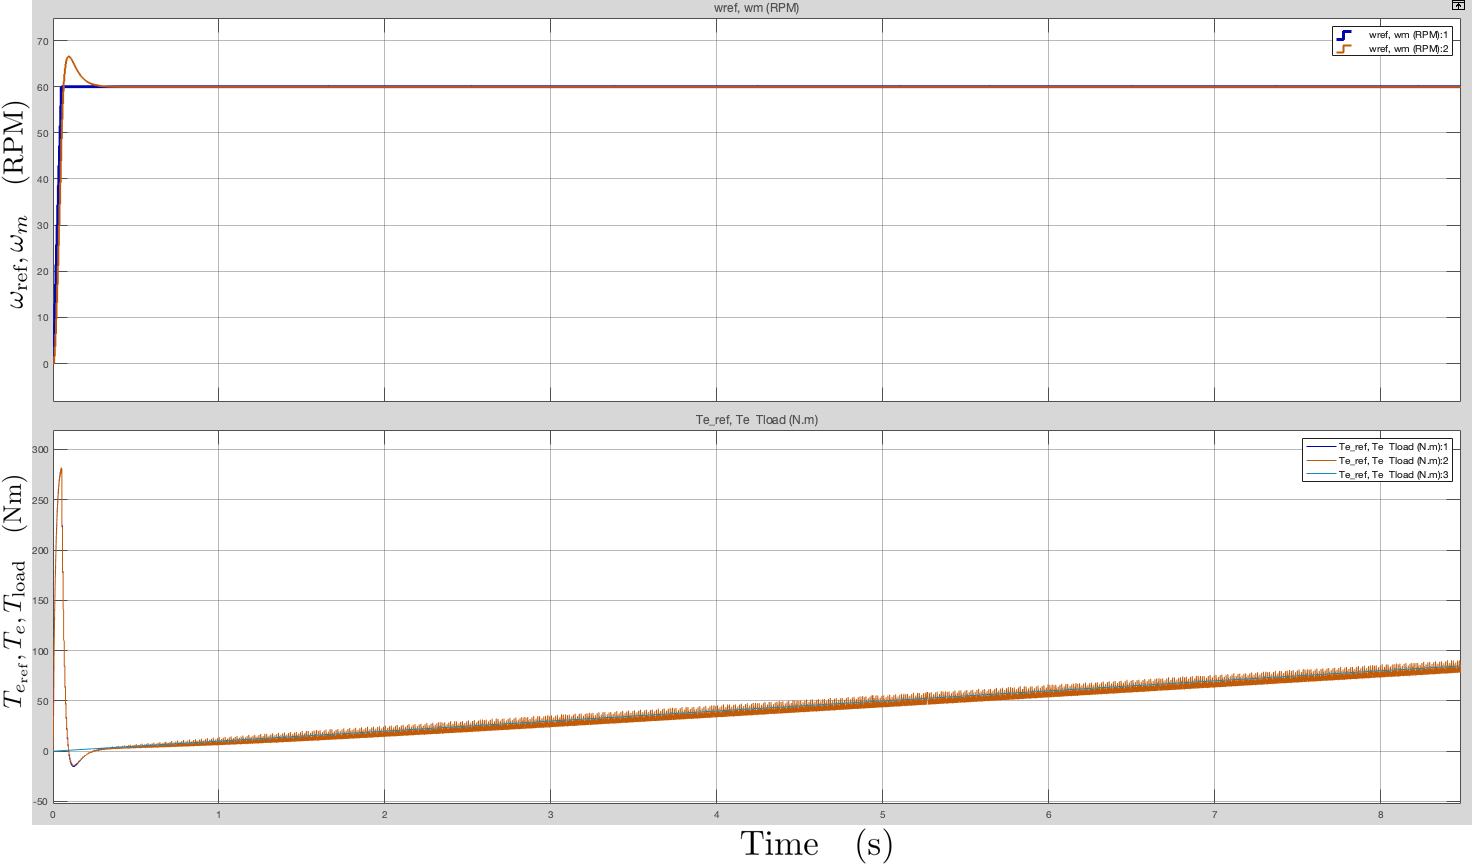
\includegraphics[width=4in]{conference/foc_60rpm.png} % Replace with your torque response comparison graph
		\caption{Torque Response of FOC with ramp input}
	\end{figure}
\end{frame}




\begin{frame}{PCB Design}
	\begin{figure}
		\centering

		\fbox{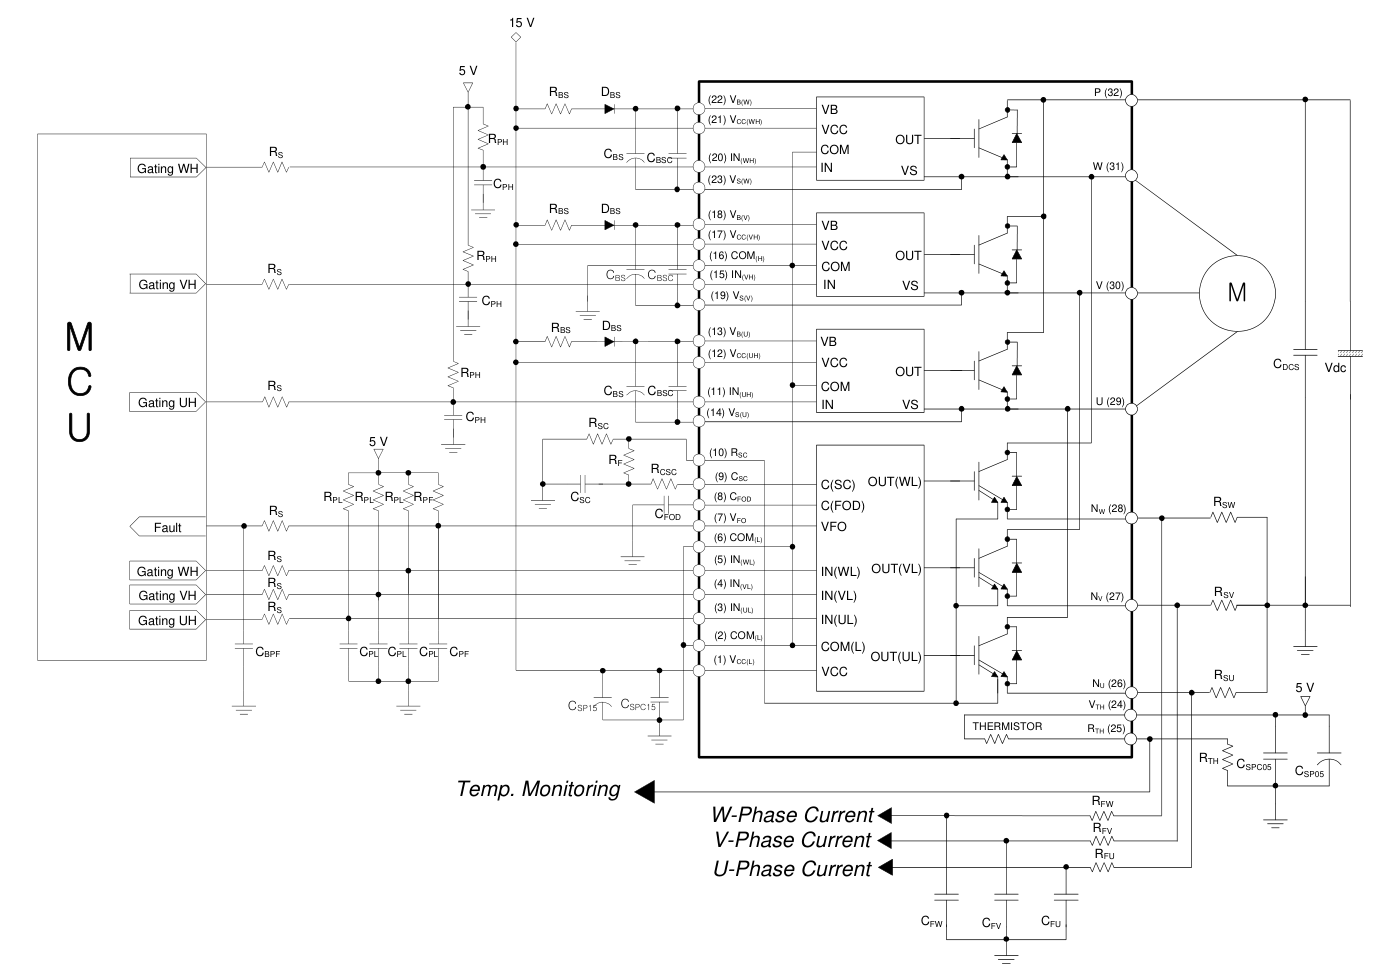
\includegraphics[width=4in]{sections/section4/images/PCBDesign/ApplicationCircuitfromDatasheet.png}}

	\end{figure}
\end{frame}


% MCU interface circuit

\begin{frame}{MCU Interface Circuit}
	\begin{figure}
		\centering

		\fbox{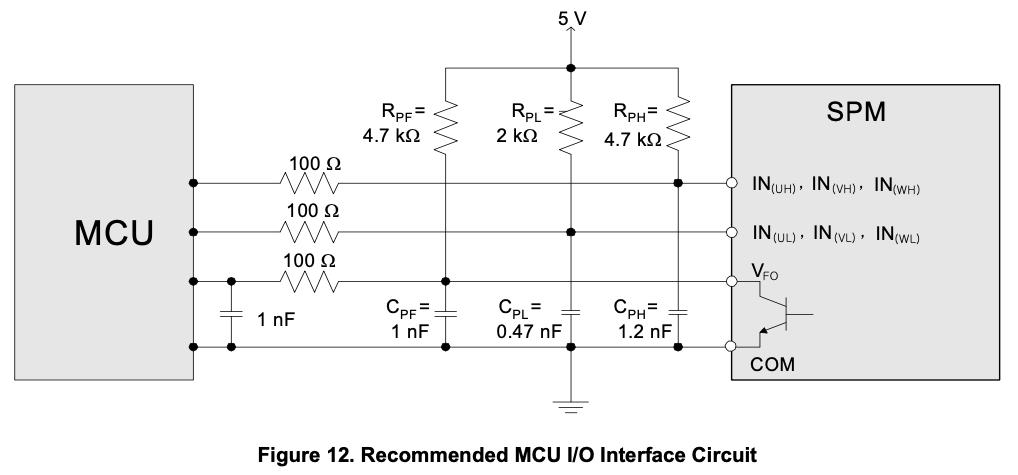
\includegraphics[width=4in]{sections/ppt/mcuInt.jpg}}

		\caption{MCU Interface Circuit}
	\end{figure}

	\begin{itemize}
		\item Bypass capacitors ground H.F. oscillations, decoupling DC circuit from A.C. Noise.
		\item Input pullup removes load strain on MCU.
	\end{itemize}
\end{frame}


% Short circuit protection circuit image

\begin{frame}{Short Circuit Protection Circuit}
	\begin{figure}
		\centering

		\fbox{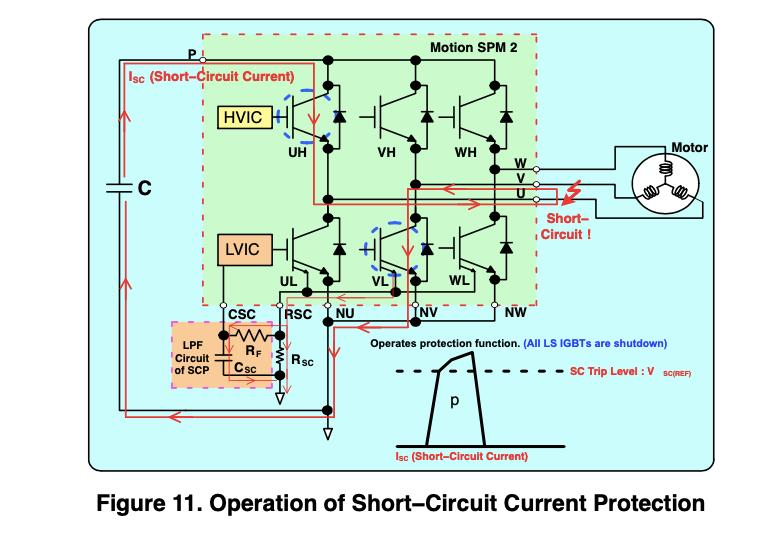
\includegraphics[width=2.8in]{sections/ppt/short-circuit-protection.jpg}}

		\caption{Short Circuit Protection Circuit}
	\end{figure}


	\begin{itemize}
		\item Seperate open-emitter pins are provided from low-side IGBTs for current sensing.
	\end{itemize}
\end{frame}



% Under voltage lockout circuit image

\begin{frame}{Under Voltage Lockout Circuit}
	\begin{figure}
		\centering

		\fbox{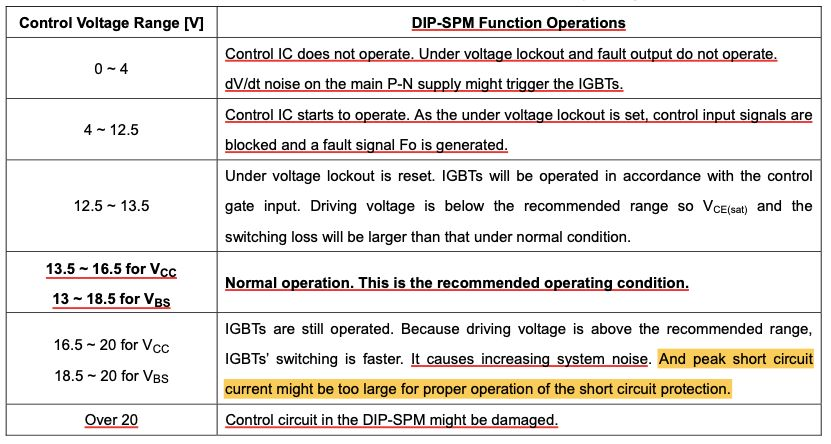
\includegraphics[width=4in]{sections/ppt/UVLC.jpg}}

		\caption{Under Voltage Lockout Circuit}
	\end{figure}
\end{frame}

% Bootstaro circyut image

\begin{frame}{Bootstrap Circuit}
	\begin{figure}
		\centering

		\fbox{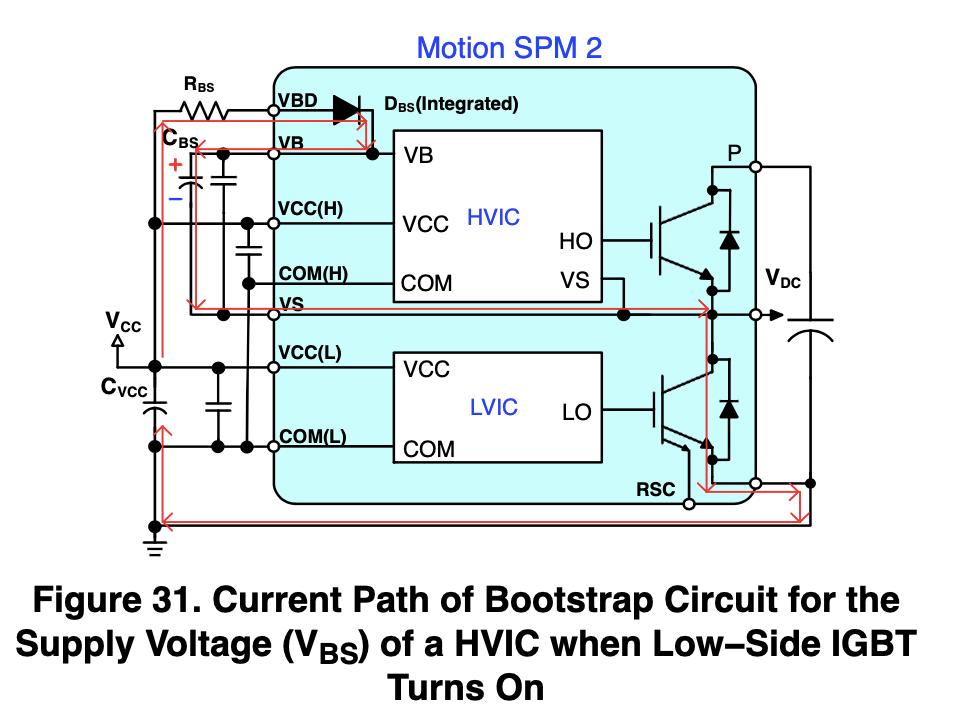
\includegraphics[width=2.8in]{sections/ppt/bootstrap.jpg}}

		\caption{Bootstrap Circuit}
	\end{figure}

	\begin{itemize}
		\item Floating Emitter
		\item Charges when low-side switch is on
	\end{itemize}
\end{frame}



% Bootstrap intial charging  graph image

\begin{frame}{Bootstrap Initial Charging}
	\begin{figure}
		\centering
		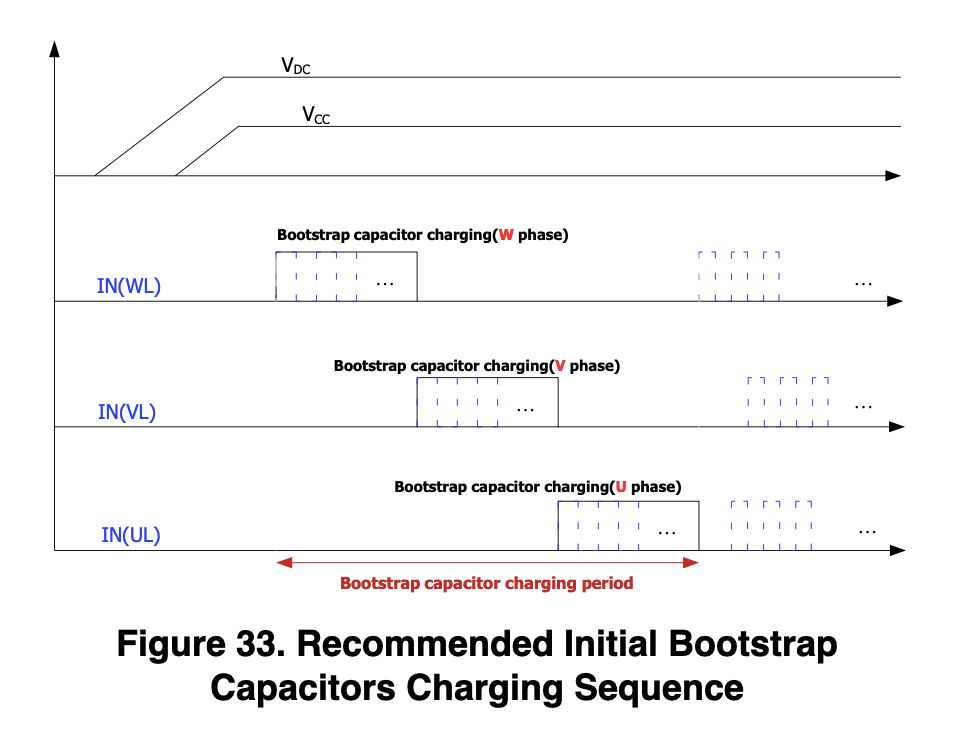
\includegraphics[width=2.6in]{sections/ppt/initalChargingGraph.jpg}
		\caption{Bootstrap Initial Charging}
	\end{figure}

	\begin{equation}
		t_\text{charge} = C_\text{BS} \times R_\text{BS} \times \frac{1}{\Delta} \times \ln\left(\frac{V_\text{CC} - V_\text{BS(min)}}{V_\text{F} - V_\text{LS}}\right)
	\end{equation}
\end{frame}

% Slide 19: PCB Layout Design in Ultiboard
\begin{frame}{PCB Layout Design}
	\begin{columns}
		\column{0.5\textwidth}
		\begin{figure}
			\centering
			\fbox{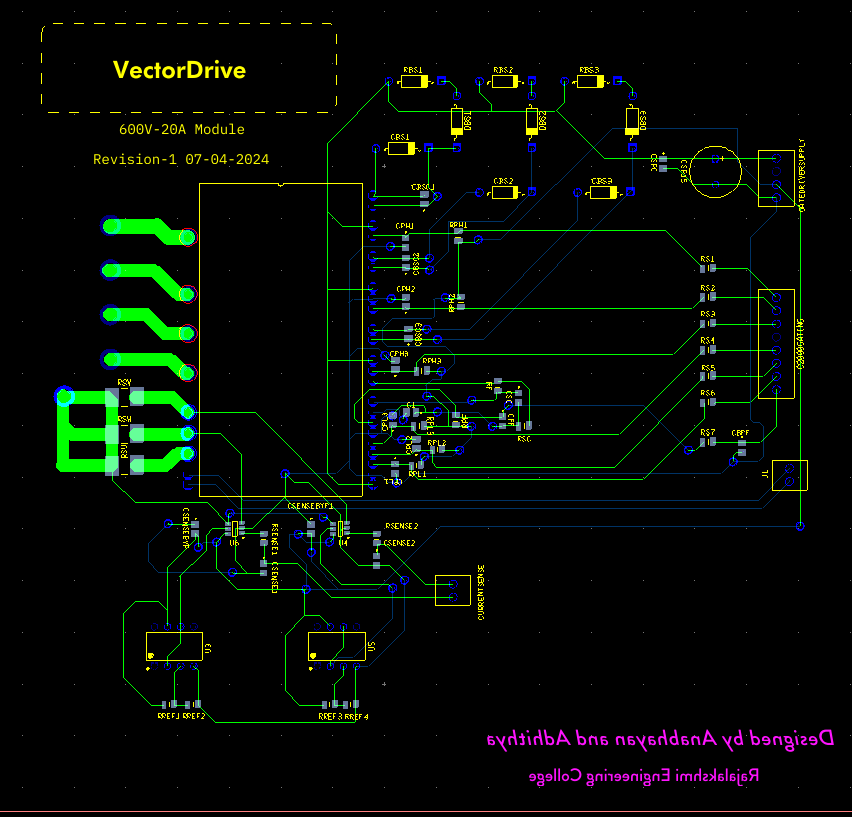
\includegraphics[width=1.8in]{sections/section4/images/PCBDesign/Ultiboard/Ultiboard.png}}
			\caption{PCB Layout Design in Ultiboard}
		\end{figure}
		\column{0.5\textwidth}
		\begin{figure}
			\centering
			\fbox{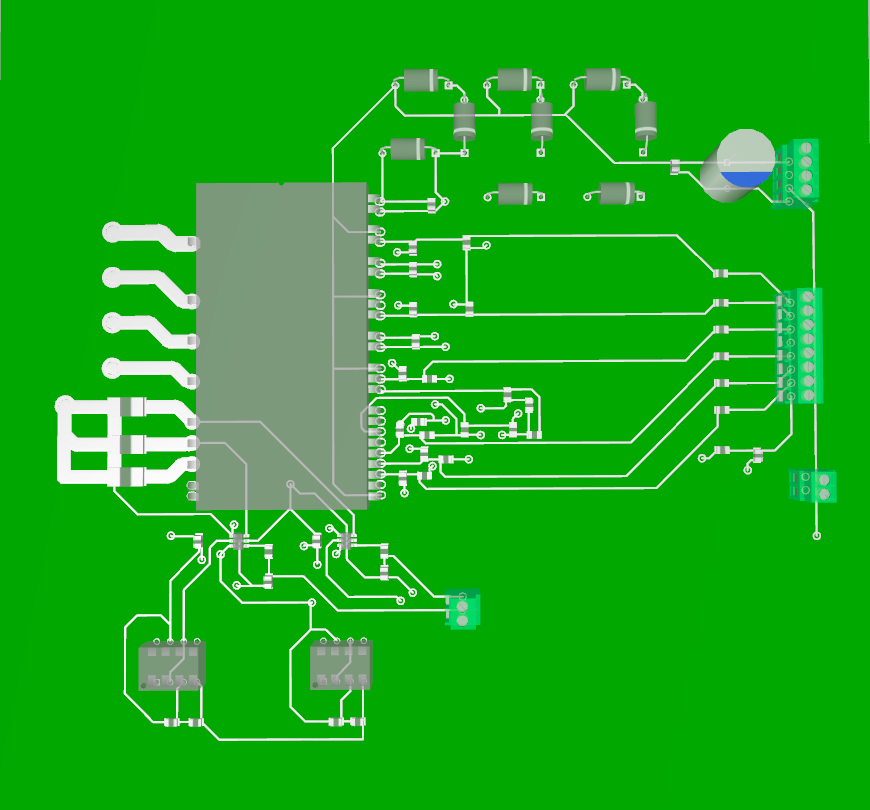
\includegraphics[width=1.8in]{sections/section4/images/PCBDesign/Ultiboard/3DTopView.png}}
			\caption{3D View of PCB Layout Design in Ultiboard}
		\end{figure}
	\end{columns}
\end{frame}

% rotor load angle image



% Current sense circuit image block diagram

\begin{frame}{Current Sensing Circuit}
	\begin{columns}
		\column{0.65\textwidth}
		\begin{figure}
			\centering
			\fbox{\includegraphics[width=2.3in]{sections/ppt/currentSense.jpg}}
			\caption{Current Sensing Circuit}

		\end{figure}
		\begin{itemize}
			\item Differential amplifier of gain $20 \frac{V}{V}$ is connected across shunt resistor and postive side DC shifted by $\frac{V_{cc}}{2}$ for bi-directional current sensing.
		\end{itemize}
		\column{0.4\textwidth}
		\begin{itemize}
			\item $I_\text{peak} = 2A \Rightarrow$

			\item $V_{out}= 10\text{mV} \cdot 20 = 0.2\text{V}$
		\end{itemize}
	\end{columns}
\end{frame}

% Slide 21: Current Sensing Circuit in Multisim
\begin{frame}{Current Measurement}
	\begin{figure}
		\centering

		\fbox{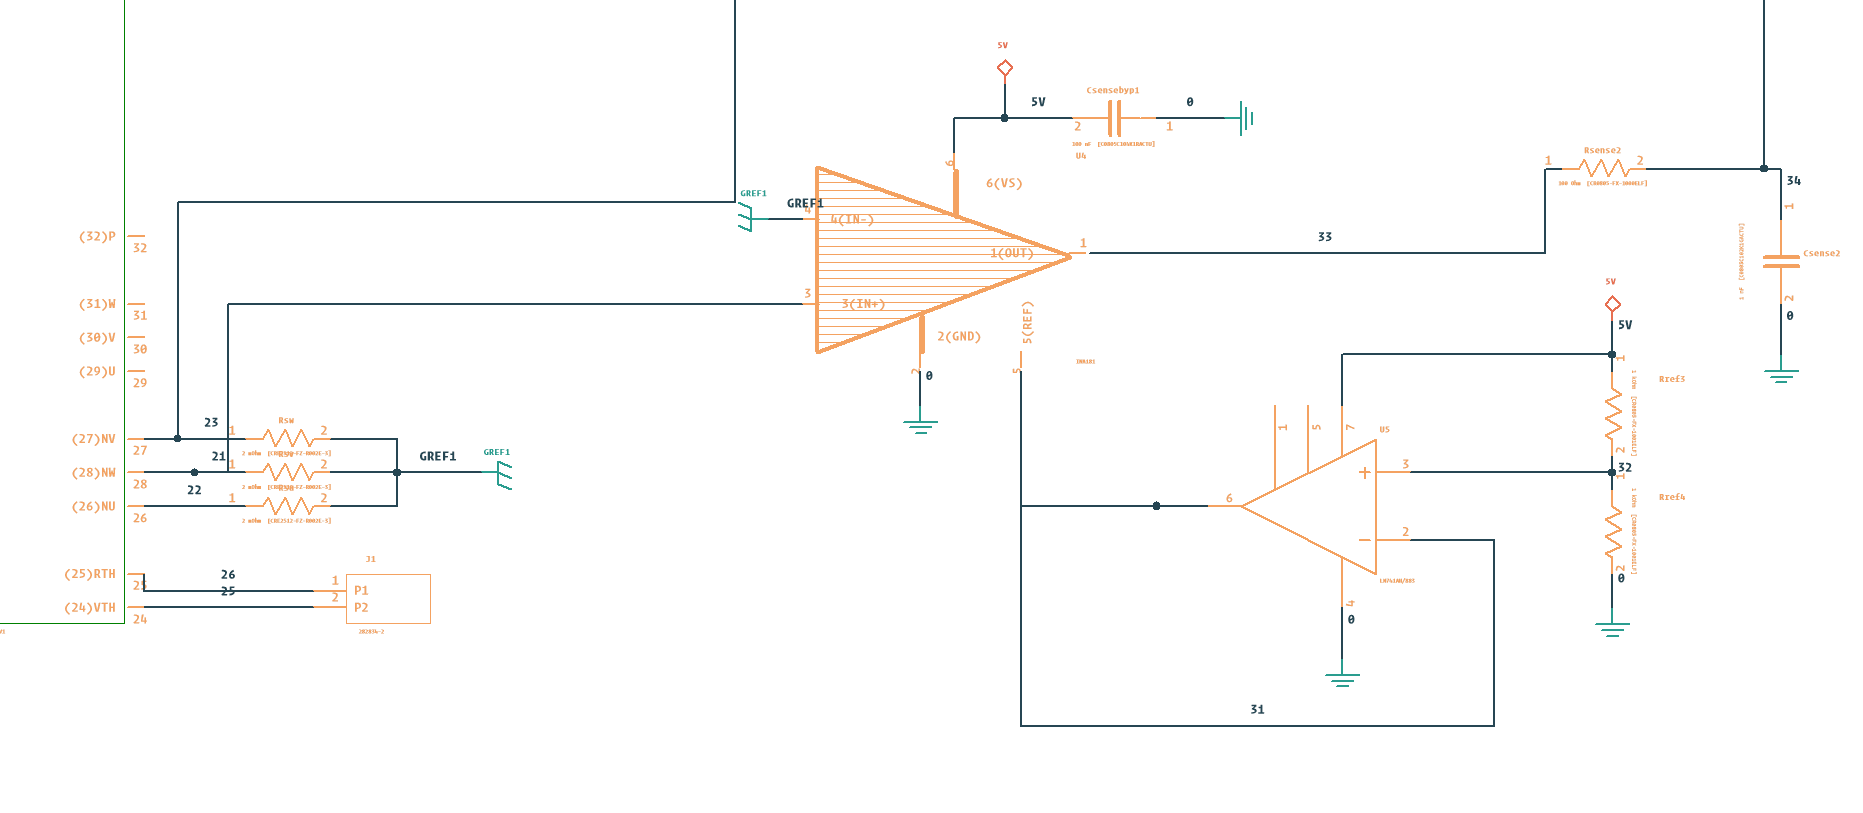
\includegraphics[width=4in]{sections/section4/images/PCBDesign/Multisim/MultisimCurrentSensing.png}}

		\caption{Current Sensing Circuit in Multisim (one phase shown)}
	\end{figure}
\end{frame}

% ePWM module block diagram

\begin{frame}{ePWM Module}
	\begin{figure}
		\centering

		\fbox{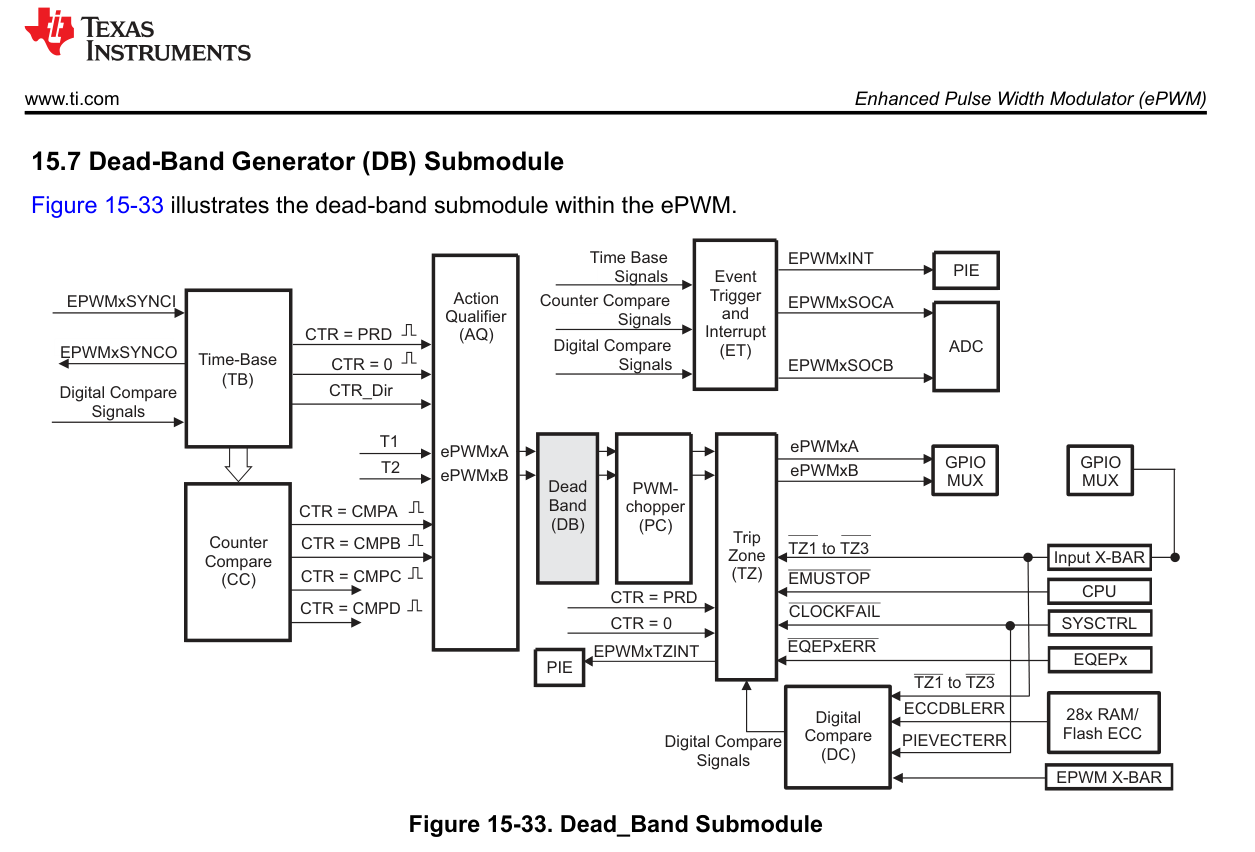
\includegraphics[width=4in]{sections/ppt/ePWM.png}}

		\caption{ePWM Module}
	\end{figure}
\end{frame}


% ePWM sub-module and it's graph

\begin{frame}{ePWM Sub-Module}
	\begin{figure}
		\centering
		\fbox{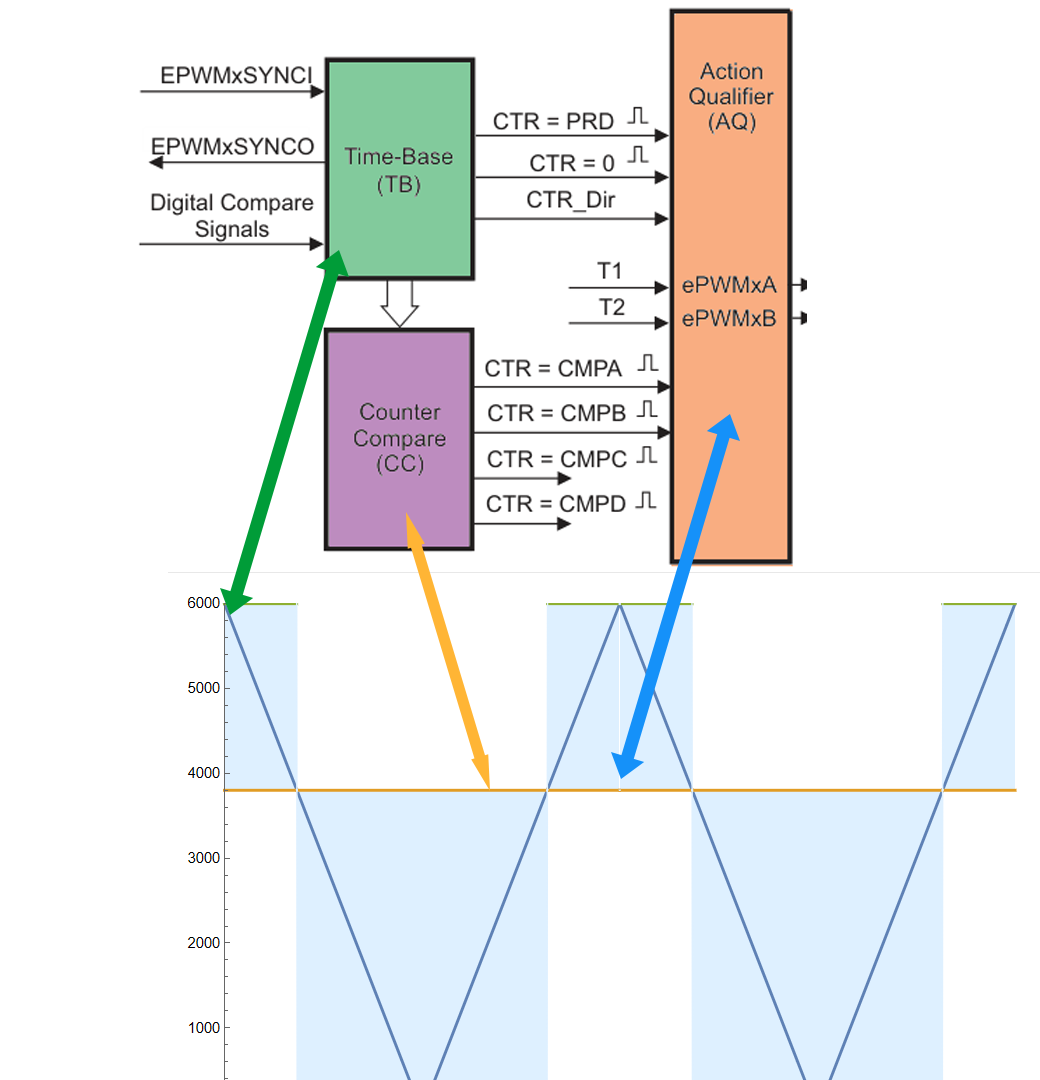
\includegraphics[width=2.5in]{sections/finalReview/ePWMEachSubmoduleGraph.png}}
		\caption{ePWM Sub-Module}
	\end{figure}
\end{frame}


% Counter compare and timer period visualtion 1

\begin{frame}{Counter Compare and Timer Period Visualization}
	\begin{figure}
		\centering
		\fbox{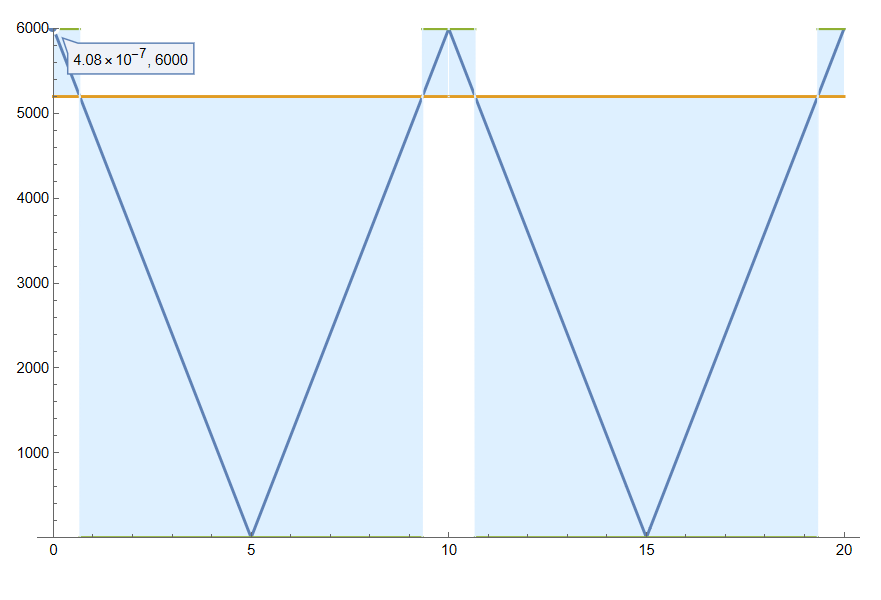
\includegraphics[width=4in]{sections/ppt/CC1.png}}
		\caption{Counter Compare High}
	\end{figure}
\end{frame}

\begin{frame}{Counter Compare and Timer Period Visualization}
	\begin{figure}
		\centering
		\fbox{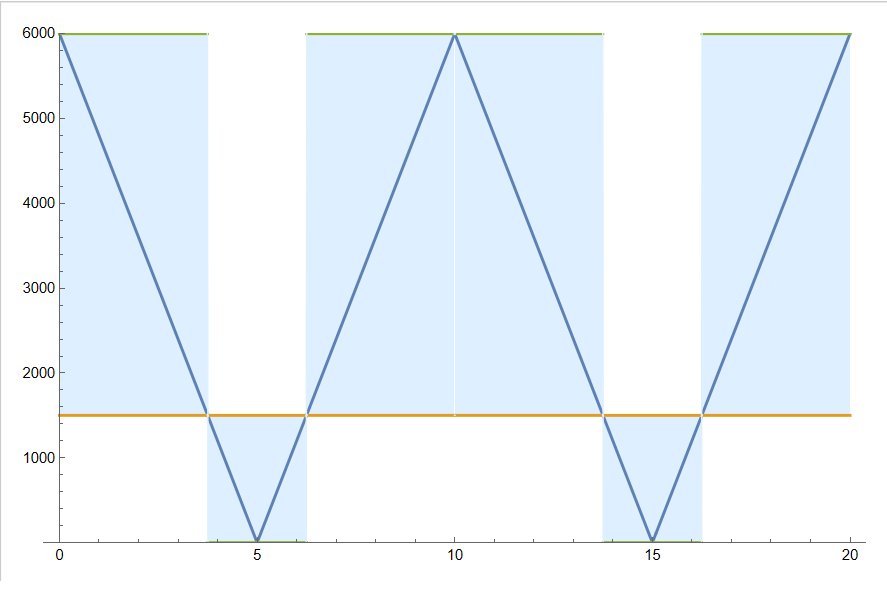
\includegraphics[width=4in]{sections/ppt/CC2.png}}
		\caption{Counter Compare Low}
	\end{figure}
\end{frame}

\begin{frame}{Counter Compare and Timer Period Visualization}
	\begin{figure}
		\centering
		\fbox{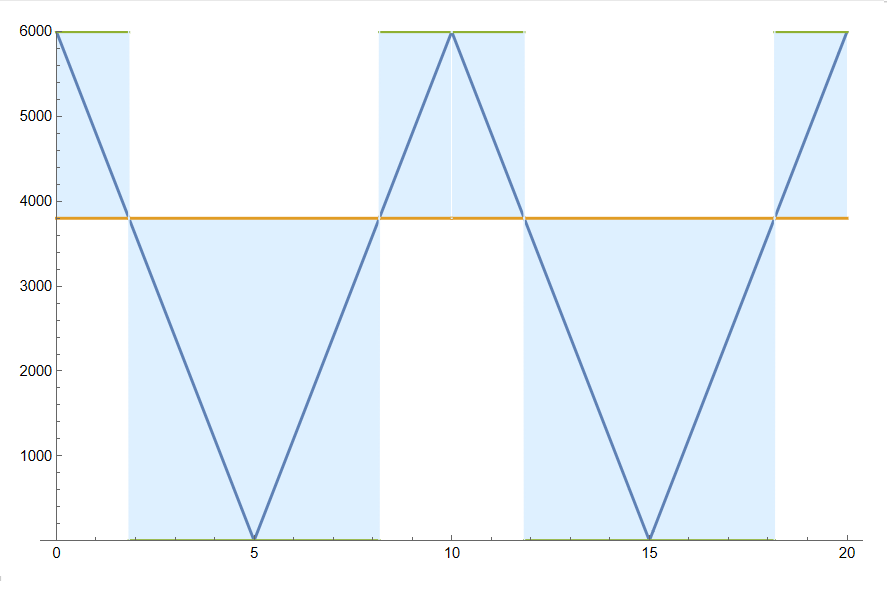
\includegraphics[width=4in]{sections/ppt/CC3.png}}
		\caption{Counter Compare half}
	\end{figure}
\end{frame}


\begin{frame}{TBPRD Calculation}

	\begin{columns}[T]
		\column{0.5\textwidth}
		\begin{itemize}
			\item PWM Frequency ($F_{PWM}$): 15 kHz (recommended by FSAM20SH60A datasheet)
			\item System Clock (SYSCLK): 200 MHz
			\item High Speed Clock Divider (HSPCLKDIV): 1
			\item Clock Divider (CLKDIV): 1
		\end{itemize}
		\column{0.5\textwidth}
		\begin{align*}
			T_{PWM}   & = \frac{1}{F_{PWM}}                      \\
			T_{TBCLK} & = \frac{SYSCLK}{HSPCLKDIV \times CLKDIV} \\
			TBPRD     & = \frac{T_{PWM}}{2 \times T_{TBCLK}}
		\end{align*}
	\end{columns}

	\vspace{0.5cm}

	\begin{align*}
		T_{PWM}   & = \frac{1}{15 \times 10^3} \text{ seconds}                               \\
		T_{TBCLK} & = \frac{200 \times 10^6}{1 \times 1} = 200 \times 10^6 \text{ Hz}        \\
		TBPRD     & = \frac{\frac{1}{15 \times 10^3}}{2 \times 200 \times 10^6} \approx 6667
	\end{align*}

	\tiny{Therefore, the Timer Period (TBPRD) is 6667.}
\end{frame}


\begin{frame}{ePWM Configuration}
	\begin{figure}
		\centering
		\fbox{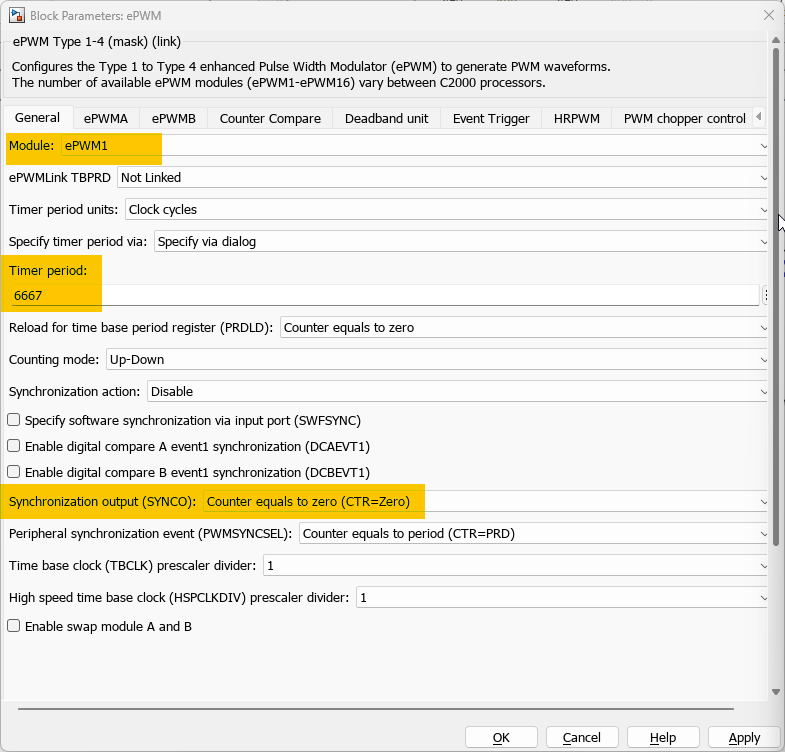
\includegraphics[width=3in]{sections/section6/images/SVPWM/ePWMTBPRD.png}}
		\caption{ePWM configuration in Simulink}
	\end{figure}
\end{frame}


% svpwm switches and states images

\begin{frame}{SVPWM Switching States}
	\begin{figure}
		\centering
		\fbox{\includegraphics[width=2.8in]{sections/finalReview/svpwmSwitches.png}}
		\caption{SVPWM Switching States}
	\end{figure}
\end{frame}

% svpwm gate pulses may look like.

\begin{frame}{SVPWM Gate Pulses}
	\begin{figure}
		\centering
		\fbox{\includegraphics[width=4in]{sections/finalReview/svpwmgatepulses.png}}
		\caption{SVPWM Gate Pulses}
	\end{figure}
\end{frame}


\begin{frame}{Space Vector Pulse Width Modulation (SVPWM)}

	\begin{figure}
		\centering
		\fbox{\includegraphics[width=2.2in]{sections/finalReview/svpwm.jpg}}
		\caption{Gate pulse generation}
	\end{figure}

	\begin{itemize}
		\item \textbf{Increased Efficiency:} SVPWM reduces harmonic distortion.
		\item \textbf{Higher Voltage Utilization:} SVPWM allows 15\% more DC bus voltage.
		\item \textbf{Reduced Switching Losses}
	\end{itemize}

\end{frame}



\begin{frame}{Open loop: SVPWM}
	\begin{figure}
		\centering
		\fbox{\includegraphics[width=4in]{sections/ppt/SVPWM_Simulink.png}}
		\caption{SVPWM Simulink Model}
	\end{figure}
\end{frame}


% Slide 28: Hardware setup with RC filter and Launchpad
\begin{frame}{SVPWM with Low Pass Filter}
	\begin{figure}
		\centering

		\fbox{\includegraphics[width=4in]{sections/section6/images/SVPWM/LPFandC2000.jpg}}

		\caption{Hardware setup with RC filter and Launchpad}
	\end{figure}
\end{frame}

% Slide 29: Output of SVPWM with low pass filter
\begin{frame}{Output of SVPWM with LPF}
	\begin{figure}
		\centering

		\fbox{\includegraphics[width=4in]{sections/section6/images/SVPWM/SVPWM2phases.jpg}}

		\caption{Output of SVPWM with low pass filter}
	\end{figure}
\end{frame}


% Slide 30: Dead band time
\begin{frame}{Dead Band Configuration}
	\begin{figure}
		\centering

		\fbox{\includegraphics[width=4in]{sections/section6/images/SVPWM/DeadBand20Us.jpeg}}
		\caption{Dead band time}
	\end{figure}
\end{frame}





% Slide for DC Bus
\begin{frame}{DC Bus Setup}
	\begin{figure}
		\centering
		\fbox{\includegraphics[width=3in]{sections/section6/images/hardwareSetup/DC bus rectifier transformer.jpg}
		}\caption{DC Bus Setup: 230V AC to 48V DC conversion with capacitor banks for stable power delivery}
	\end{figure}
\end{frame}

% Slide for Inverter and Controller
\begin{frame}{Inverter and Controller}
	\begin{figure}
		\centering
		\fbox{\includegraphics[width=2.3in]{sections/section6/images/hardwareSetup/IPM and C2000.jpg}
		}\caption{Inverter (FSAM20SH60A) and Controller (F28379D Launchpad) Setup}
	\end{figure}
\end{frame}

% Slide for Full Setup
\begin{frame}{Complete Hardware Setup}
	\begin{figure}
		\centering
		\fbox{\includegraphics[width=3in]{sections/section6/images/hardwareSetup/fullSetupWithMotorAndIPM.jpg}
		}\caption{Experimental Setup for Motor Control System with Induction Motor, DC Bus, Inverter, and Controller}
	\end{figure}
\end{frame}

\begin{frame}{Challenges: False Positives from Fault Alarm}

	\begin{figure}
		\centering
		\fbox{\includegraphics[width=4in]{sections/section6/images/hardwareSetup/VccNoiseAndFaultAlarm.jpg}
		}\caption{Vcc Noise and Fault Alarm Signal}
	\end{figure}

	\begin{itemize}
		\item Top waveform: Vcc voltage (power supply for IPM control)
		\item Bottom waveform: Fault alarm signal (triggered by noise on Vcc)
	\end{itemize}

\end{frame}
\begin{frame}{Mitigation Strategies}

	\begin{itemize}
		\item \textbf{Isolation Attempts:}
		      \begin{itemize}
			      \item Separate control and power stage grounds using separate transformers and rectifiers.
			      \item Temporarily shorted RSC and CSC pins to ground to assess external noise influence.
		      \end{itemize}
		\item \textbf{Noise Reduction Techniques:}
		      \begin{itemize}
			      \item Added metal film capacitors across the DC bus to suppress switching transients.
			      \item Reduced switching frequency to minimize voltage/current change rate and noise.
		      \end{itemize}
		\item \textbf{Future Considerations:}
		      \begin{itemize}
			      \item Further noise reduction through filtering on control signals and power supply lines.
			      \item Improved PCB layout to minimize noise coupling paths and optimize component placement.
		      \end{itemize}
	\end{itemize}

\end{frame}

\begin{frame}{Conclusion}

	\begin{itemize}
		\item \textbf{Achievements:}
		      \begin{itemize}
			      \item Successful simulation of FOC system demonstrating significant performance improvements.
			      \item Design and development of hardware setup including PCB design and component integration.
			      \item Identification and analysis of challenges related to noise and false alarms.
		      \end{itemize}
		\item \textbf{Challenges:}
		      \begin{itemize}
			      \item Persistent false positives from the IPM's fault alarm despite implemented mitigation strategies.
			      \item Limited hardware validation due to the unresolved fault alarm issue.
		      \end{itemize}
		\item \textbf{Future Work:}
		      \begin{itemize}
			      \item Explore additional noise reduction techniques and PCB layout optimization.
			      \item Investigate alternative IPM modules or fault detection mechanisms.
			      \item Implement and validate the closed-loop FOC system in hardware upon resolving the challenges.
		      \end{itemize}
	\end{itemize}

\end{frame}


\begin{frame}{Literature Review}
	\begin{center}

		\begin{table}
			\centering
			\tiny
			\rowcolors{2}{blue!74}{black!80} % this command adds alternating color for rows
			\begin{tabular}{|p{1.4cm}|p{2.cm}|c|p{6cm}|}
				\hline
				\rowcolor{yellow} % this command changes the header color to yellow

				\textcolor{black}{\textbf{Author}}         & \textcolor{black}{\textbf{Title}}                                                                       & \textcolor{black}{\textbf{Year}} & \textcolor{black}{\textbf{Summary}}                                                                                                                                                                                                                                                                                                                                               \\

				\hline
				\vspace{0.005in} E.S.Tez                   & \vspace{0.005in} A Simple Understanding Of Field Orientation For Ac Motor Control                       & \vspace{0.01in} 1995             & \vspace{0.005in} \RaggedRight The article teaches field-orientation for AC motor control, which aligns the stator and rotor fields for fast torque control. It corrects some wrong ideas about motor models and parameters, and shows a new field-orientation design called INVECTER.                                                                                             \\
				\hline
				\vspace{0.1in}
				\vspace{0.005in}  Wenzhuo Chen et.al       & \vspace{0.005in}  Simulation of Permanent Magnet Synchronous Motor Field oriented Vector Control System & 2014                             & \vspace{0.04in} \RaggedRight The text describes coordinate conversion's role in managing motor currents, especially excitation and torque. It highlights PI controllers and SVPWM pulses for precise control of PMSM. Simulation results validate the vector control method's accuracy, supporting real-world system design.\vspace{0.04in}                                       \\
				\hline
				\vspace{0.005in}  Dianguo Xu  et.al        & \vspace{0.005in}  A Review of Sensorless Control Methods for AC Motor Drives                            & 2018                             & \vspace{0.04in} \RaggedRight Sensorless control - signal injection methods are simpler and easier to execute than model reference adaptive system and Kalman filter. Requires large amount of data. \vspace{0.04in}                                                                                                                                                               \\
				\hline

				\vspace{0.005in}  Rupprecht Gabriel. et al & \vspace{0.005in} Implementation of Field Oriented Control for Permanent Magnet Synchronous Motor        & 1980                             & \vspace{0.04in} \RaggedRight The article shows how microprocessors can control AC machines better with field orientation, which improves their dynamic performance. It gives the theory of AC motor control by field orientation and some results from a test drive. It explains the induction motor model and talks about the future possibilities in the field. \vspace{0.04in} \\
				\hline
				\vspace{0.005in}  Arun Dominic Dn et.al    & Analysis of field-oriented controlled induction motor drives overview of sensorless scheme              & 2014                             & \vspace{0.04in} \RaggedRight This article  explores use of blanking periods and space vector modulation to enhance low-speed drive performance, providing a thorough technique review.                                                                                                                                                                                            \\
				\hline
			\end{tabular}
			\label{tab:lit-survey}
		\end{table}
	\end{center}
\end{frame}

\end{document}